\documentclass[nojss]{jss}

%% -- LaTeX packages and custom commands ---------------------------------------
%\VignetteIndexEntry{sstvars: Structural Smooth Transition Vector Autoregressive Models R}

%% recommended packages
\usepackage{thumbpdf, lmodern}

%% Packages added by the author
\usepackage{amsmath} % \align, etc.
\usepackage{amssymb} % \mathbb, etc.
\usepackage{mathtools} % matrix*: [c] centered, [l] left-aligned, [r] right-aligned

%% new custom commands
\newcommand{\class}[1]{`\code{#1}'}
\newcommand{\fct}[1]{\code{#1()}}
\newtheorem{condition}{Condition}
\newtheorem{proposition}{Proposition}
\newtheorem{assumption}{Assumption}


%% For Sweave-based articles about R packages:
%% need no \usepackage{Sweave}



%% -- Article metainformation (author, title, ...) -----------------------------

%% - \author{} with primary affiliation (and optionally ORCID link)
%% - \Plainauthor{} without affiliations
%% - Separate authors by \And or \AND (in \author) or by comma (in \Plainauthor).
%% - \AND starts a new line, \And does not.
\author{Savi Virolainen\\ University of Helsinki}
\Plainauthor{Savi Virolainen}

%% - \title{} in title case
%% - \Plaintitle{} without LaTeX markup (if any)
%% - \Shorttitle{} with LaTeX markup (if any), used as running title
\title{sstvars: Structural Smooth Transition Vector Autoregressive Models in \proglang{R}}
\Plaintitle{sstvars: Structural Smooth Transition Vector Autoregressive Models in R}
\Shorttitle{Structural Smooth Transition Vector Autoregressive Models \proglang{R}}

%% - \Abstract{} almost as usual
\Abstract{
  We describe the \proglang{R} package \pkg{sstvars}, which provides tools for estimating and analyzing the reduced form and structural smooth transition vector autoregressive (STVAR) models. This includes also threshold vector autoregressive models. The package implements various transition weight functions, conditional distributions, identification methods, and parameter restrictions. The model parameters are estimated with the method of maximum likelihood by running multiple rounds of a two-phase estimation procedure in which a genetic algorithm is used to find starting values for a gradient based variable metric algorithm. For evaluating the adequacy of the estimated models, \pkg{sstvars} utilizes residuals based diagnostics and provides functions for graphical diagnostics and for calculating formal diagnostic tests. \pkg{sstvars} also accommodates the estimation of linear impulse response functions, nonlinear generalized impulse response functions, and generalized forecast error variance decompositions. Further functionality includes hypothesis testing, plotting the profile log-likelihood functions about the estimate, simulation from STVAR processes, and forecasting, for example. We illustrate the use of \pkg{sstvars} with a quarterly series consisting of two U.S. variables: the percentage change of real GDP and the percentage change of GDP implicit price deflator.}

%% - \Keywords{} with LaTeX markup, at least one required
%% - \Plainkeywords{} without LaTeX markup (if necessary)
%% - Should be comma-separated and in sentence case.
\Keywords{smooth transition vector autoregressive model, structural smooth transition vector autoregressive model, regime-switching,
SVAR, STVAR, maximum likelihood estimation}
\Plainkeywords{smooth transition vector autoregressive model, structural smooth transition vector autoregressive model, regime-switching,
SVAR, STVAR, maximum likelihood estimation}

%% - \Address{} of at least one author
%% - May contain multiple affiliations for each author
%%   (in extra lines, separated by \emph{and}\\).
%% - May contain multiple authors for the same affiliation
%%   (in the same first line, separated by comma).
\Address{
  Savi Virolainen\\
  Faculty of Social Sciences\\
  University of Helsinki\\
  P. O. Box 17, FI-0014 University of Helsinki, Finland\\
  E-mail: \email{savi.virolainen@helsinki.fi}
}


\begin{document}

\section{Introduction}
Linear vector autoregressive (VAR) models are a standard tools in time series econometrics. They can be employed to answer questions about the statistical relationships of different variables or to forecast future values of the process, for example. Structural VAR models, in particular, allow to trace out the effects of economic shocks. With an appropriate choice of the autoregressive order $p$, a linear VAR model is often able to filter out autocorrelation from the series very well. If the errors are assumed to follow an autoregressive conditional heteroskedasticity (ARCH) process, the model is also often able to adequately filter out conditional heteroskedasticity from the series.

In some cases, linear VAR models are not, however, capable of capturing all the relevant characteristics of the data. This includes shifts in the mean or volatility, and changes in the autoregressive dynamics of the process. Such nonlinear features frequently occur in economic time series when the underlying data generating dynamics vary in time, for example, depending the specific state of the economy. Various types of time series models capable of capturing this kind of regime-switching behavior have been proposed, one of them is the smooth transition vector autoregressive (STVAR) models that allow to capture gradual shifts in the dynamics of the data. They consist of a finite number of regimes, each of which are linear vector autoregressions that are characterized by different autoregressive coefficients or error term covariance matrices. The package \pkg{sstvars} considers STVAR models in which, at each point of time, the observation is a weighted average of the conditional means of the regimes plus a random error whose covariance matrix is a weighted average of the covariance matrices of the regimes. The weights, in turn, are expressed in terms of time-varying transition weights that depend on the preceding observations. Different STVAR models can be created by specifying the transition weights or the error distribution in various ways.

This manuscript describes the \proglang{R} package \pkg{sstvars} providing a set of easy-to-use tools for STVAR modeling, including also threshold vector autoregressive models. There are tools for unconstrained and constrained maximum likelihood (ML) estimation of the model parameters, residual based model diagnostics, estimation of linear impulse response functions, nonlinear generalized impulse response functions, and generalized forecast error variance decompositions. Further functionality includes hypothesis testing, plotting the profile log-likelihood functions about the estimate, simulation from STVAR processes, and forecasting, for example. Various transition weight functions are accommodated, including exogenous weights, logistic weights \citep{Anderson+Vahid:1998}, multinomial logit weights, exponential weights \citep[e.g.,][]{Hubrich+Terasvirta:2013}, threshold weights \citep{Tsay:1998}, and transition weights that defined as weighted relative likelihoods of the regimes corresponding to the preceding $p$ observations \citep{Lanne+Virolainen:2024}. Currently, the accommodated conditional distributions include Gaussian distribution, Student's $t$ distribution, and Student's $t$ distribution with independent components, whereas the accommodated identification methods include recursive identification, identification by heteroskedasticity \citep{Lutkepohl+Netsunajev:2017}, and identification by non-Gaussianity \citep{Virolainen2:2024}.

The estimation of the model parameters can, in some cases, be rather tricky. Particularly when the transition weights are determined endogenously, there is a very large number of modes to the log-likelihood function, and large areas of the parameter space, where the log-likelihood function is flat in multiple directions. Therefore, the model parameters are estimated by running multiple rounds of a two-phase estimation procedure in which a modified genetic algorithm is used to find starting values for a gradient based variable metric algorithm. Because of the multimodality of the log-likelihood function, some of the estimation rounds may end up in different local maximum points, thereby enabling the researcher to build models not only based on the global maximum point but also on the local ones. The estimated models can be conveniently examined with the \code{summary} and \code{plot} methods.

The remainder of this paper is organized as follows. Section~\ref{sec:models} defines the implemented reduced form STVAR models and discusses some of their properties. Section~\ref{sec:struct_stvar} discusses the accommodated structural STVAR models and discusses identification of the structural shocks. Section~\ref{sec:estimation} discusses estimation of the model parameters. We also illustrate how the STVAR models can be estimated and examined with \pkg{sstvars} and how various parameter restrictions can be imposed in the estimation. Section~\ref{sec:res} discusses how to evaluate the model adequacy with \pkg{sstvars} using residual based diagnostics. Section~\ref{sec:impulseresponse} discusses impulse response analysis, including generalized impulse response functions and generalized forecast error variance decompositions. Section~\ref{sec:STVAR} shows how the STVAR models can be constructed with given parameter values. In Section~\ref{sec:simufore}, we first show how to simulate observations from a STVAR process, and then we illustrate how to forecast future values of a STVAR process with a simulation-based Monte Carlo method. Finally, Section~\ref{sec:summary} concludes and collects some useful functions in \pkg{sstvars} to a single table for convenience. Throughout this paper, we illustrate the use of \pkg{sstvars} with a quarterly series consisting of two U.S. variables: the percentage change of real GDP and the percentage change of GDP implicit price deflator, covering the period from 1959Q1 to 2019Q4.

\section{Smooth Transition Vector Autoregressive Models}\label{sec:models}
This section describes the STVAR models implemented in \pkg{sstvars}. First, we describe the general framework of STVAR models accommodated by \pkg{sstvars} and present a sufficient condition for their ergodic stationarity. Then, we present the implemented specifications of transition weight functions and conditional distributions. Finally, we discuss structural STVAR models and implemented methods for identification of the shocks.

\subsection{General framework for STVAR models}\label{sec:genstvar}
Let $y_t$, $t=1,2,...$, be the $d$-dimensional time series of interest and $\mathcal{F}_{t-1}$ denote the $\sigma$-algebra generated by the random vectors $\lbrace y_{t-j}, j>0 \rbrace$. We consider STVAR models with $M$ regimes and autoregressive order $p$ assumed to satisfy
\begin{align}
y_t &=\sum_{m=1}^M \alpha_{m,t}\mu_{m,t} + u_t, \quad u_{t} \sim MD(0, I_d)\label{eq:stvar1} \\
\mu_{m,t} &= \phi_{m,0} + \sum_{i=1}^{p}A_{m,i}y_{t-i}, \quad m=1,...,M,\label{eq:stvar2}\\
B_tB_t' &= \sum_{m=1}^M \alpha_{m,t}\Omega_m, \label{eq:stvar3}
\end{align}
where $\phi_{m,0}\in\mathbb{R}^{d}$ are intercept parameters, $A_{m,i}$ is the lag $i$ autoregression matrix  of Regime $m$, and $u_t$ is a martingale difference sequence of reduced form innovations. %$\Omega_1,...,\Omega_M$ are the positive definite $(d\times d)$ covariance matrices of the regimes, $B_t$ is an invertible ($d\times d$) impact matrix that governs the contemporaneous relationships of the shocks and is a function of $\lbrace y_{t-j}, j=1,...,p \rbrace$. For the reduced form model, any invertible matrix $B_t$ that satisfies Equation~(\ref{eq:stvar3}) can be assumed without loss of generality, whereas structural models assume a specific structure on $B_t$. The structural errors $e_{t}$ $(d\times 1)$ are independent and identically distributed with mean zero and identity covariance matrix, and they are independent of $\mathcal{F}_{t-1}$.
The transition weights $\alpha_{m,t}$ are assumed to be $\mathcal{F}_{t-1}$-measurable functions of $\lbrace y_{t-j}, j=1,...,p \rbrace$ and to satisfy $\sum_{m=1}^{M}\alpha_{m,t}=1$ at all $t$. They express the proportions of the regimes the process is on at each point of time, and how the process shifts between the regimes. Through, a STVAR model with autoregressive order $p$ and $M$ regimes is referred to as a STVAR($p,M$) model, whenever the order of the model needs to be emphasized.

Conditional on $\mathcal{F}_{t-1}$, the conditional mean of the above described process is $\mu_{y,t} \equiv E[y_t|\mathcal{F}_{t-1}] = \sum_{m=1}^M \alpha_{m,t}\mu_{m,t}$. The conditional mean is thereby a weighted sum the regime-specific means $\mu_{m,t}$ with the weights given by the transition weights $\alpha_{m,t}$ The specification of the conditional covariance matrix $\Omega_{y,t}\equiv \text{Cov}(y_t|\mathcal{F}_{t-1})=\text{Cov}(u_t|\mathcal{F}_{t-1})$ depends on the error term distribution. The it assumed to be either Gaussian or $t$-distributed (in the conventional way), the conditional covariance matrix is assumed to be the weighted average of the covariance matrices of the regimes:
\begin{equation}
\Omega_{y,t} = \sum_{m=1}^M \alpha_{m,t}\Omega_m,
\end{equation}
where $\Omega_1,...,\Omega_M$ are the positive definite $(d\times d)$ covariance matrices of the regimes. If the error term distribution is Student's $t$ distribution with mutually independent components (hereafter independent $t$-distribution), the conditional covariance matrix is different, because the model is directly parametrized with the invertible $(d\times d)$ impact matrices $B_m$ of the regimes. In this case, the conditional covariance is matrix is:
\begin{equation}\label{eq:condcovmat}
\Omega_{y,t} = \left(\sum_{m=1}^M \alpha_{m,t}^{1/2}B_m \right) \left(\sum_{m=1}^M \alpha_{m,t}^{1/2}B_m \right)' = \sum_{m=1}^M \alpha_{m,t}\Omega_m +  \sum_{m=1}^M\sum_{n=1,n\neq m}^M\alpha_{m,t}^{1/2}\alpha_{n,t}^{1/2}\Omega_{m,n},
\end{equation}
where $\Omega_m\equiv B_mB_m'$ and $\Omega_{m,n}\equiv B_mB_n'$.

Different STVAR models are obtained by specifying the transition weights or the error distribution (i.e., the conditional distribution) in various ways. See \cite{Hubrich+Terasvirta:2013} for a survey on STVAR literature, including formulations more general than our framework. The package \pkg{sstvars} accommodates completely exogenous transition weight functions as well as transition weights are functions of $\lbrace y_{t-j}, j=1,...,p \rbrace$. In the latter case, the stationarity condition presented below applies. Moreover, $\mathcal{F}_{t-1}$-measurability of the transition weights ensures that the true generalized impulse responses functions \citep{Koop+Pesaran+Potter:1996} can be easily estimated, as completely exogenous switching-variables are excluded from affecting the weights. We also assume that the transition weights are identical for all the individual equations in (\ref{eq:stvar1}) and (\ref{eq:stvar3}), which is also required for applicability of the stationarity condition. Consequently, at each $t$‚ the process can be described as a weighted sum of linear vector autoregressions.

\subsubsection{Stationarity condition}\label{sec:stationarity}
Excluding models with exogenous transition weights, it can be shown that a sufficient condition for the ergodic stationarity of the STVAR model (\ref{eq:stvar1})-(\ref{eq:stvar3}) can expressed in terms of the joint spectral radius (JSR) of certain matrices \citep{Kheifets+Saikkonen:2020}. The JSR of a finite set of square matrices $\mathcal{A}$ is defined by
\begin{equation}
\rho(\mathcal{A}) = \underset{j\rightarrow \infty}{\limsup}\left(\underset{A\in \mathcal{A}^j}{\sup}\rho(A) \right)^{1/j},
\end{equation}
where $\mathcal{A}^j=\lbrace A_1A_2...A_j:A_i\in\mathcal{A}\rbrace$ and $\rho(A)$ is the spectral radius of the square matrix $A$.

Consider the companion form AR matrices of the regimes defined as
\begin{equation}\label{eq:boldA}
\boldsymbol{A}_m =
\underset{(dp\times dp)}{\begin{bmatrix}
A_{m,1} & A_{m,2} & \cdots & A_{m,p-1} & A_{m,p} \\
I_d  & 0     & \cdots & 0            & 0 \\
0     & I_d  &             & 0            & 0 \\
\vdots &   & \ddots & \vdots    & \vdots \\
0     & 0     & \hdots & I_d         & 0
\end{bmatrix}}, \
m=1,...,M.
\end{equation}
\citet[][Theorem 1]{Kheifets+Saikkonen:2020} and \cite{Lanne+Virolainen:2024} \citep[see also][]{Saikkonen:2008} show that if the following condition holds, the STVAR process is ergodic stationary (both strictly and second-order).
\begin{condition}\label{cond:sufficient}
$\rho(\lbrace \boldsymbol{A}_1,...,\boldsymbol{A}_M \rbrace) < 1$.
\end{condition}

Condition~\ref{cond:sufficient} is, however, computationally demanding the check in practice with a reasonable accuracy \citep[e.g.,][]{Chang+Blondel:2013}, making it impractical to use in the estimation. Therefore, we consider a necessary condition for Condition~\ref{cond:sufficient} that is easier to check in practice, which is that the usual stability condition is satisfied for each of the regimes. Specifically, the following condition, which is analogous to Corollary~1 of \cite{Kheifets+Saikkonen:2020}, is necessary for Condition~\ref{cond:sufficient}.
\begin{condition}\label{cond:necessary}
$\max\lbrace \rho(\boldsymbol{A}_1),...,\rho(\boldsymbol{A}_M)\rbrace<1$,
\end{condition}
where $\rho(\boldsymbol{A}_m)$ is the spectral radius of $\boldsymbol{A}_m$, $m=1,...,M$.

Note that validity Condition~\ref{cond:necessary} does not imply the validity of Condition~\ref{cond:sufficient}, which guarantees ergodic stationarity of the model. However, in practice models that satisfy Condition~\ref{cond:necessary} and are not very close to breaking this condition usually satisfy Condition~\ref{cond:sufficient}. For checking the validity of Condition~\ref{cond:sufficient}, \pkg{sstvars} implements (the function \code{bound_JSR}) implements the branch-and-bound method by \cite{Gripenberg:1996}. For large models Gripenberg's method may, however, take very long if tight bounds are required. Other implementations of methods bounding the JSR include the \proglang{MATLAB} toolbox \pkg{JSR} by \cite{Jungers:2023}, which automatically combines several methods and finds accurate bounds faster than \pkg{sstvars}.

\subsection{Specifications of the conditional distribution}\label{sec:cond_dist}
Currently, \pkg{sstvars} accommodates two types of error distributions: Gaussian distribution, Student's $t$, and independent Student's $t$ distribution, which are discussed below.

\subsubsection{Gaussian distribution}
Assuming the structural errors $e_t$ have standard normal distributions, the conditional distribution of $y_t$ conditional on $\mathcal{F}_{t-1}$ is Gaussian and characterized by the density function
\begin{equation}
f(y_t|\mathcal{F}_{t-1}) = n_d(y_t;\mu_{t},\Omega_{t})=(2\pi)^{-d/2}\det(\Omega_t)^{-1/2}\exp\left\lbrace -\frac{1}{2}(y_t - \mu_t)'\Omega_t^{-1}(y_t - \mu_t) \right\rbrace .
\end{equation}
That is, the conditional distribution is simply the $d$-dimensional Gaussian distribution with mean $\mu_t$ and covariance matrix $\Omega_t$. The Gaussian distribution simple and can be used with all of our transition weight functions, but in some cases it is useful to employ the more heavy tailed Student's $t$ distribution instead.

\subsubsection{Student's $t$ distribution}\label{sec:student}
To accommodate more heavy tailed data, instead of using Gaussian errors one may consider Student's $t$ errors and assume the shocks $e_t$ are Student's $t$ distributed with the mean zero, identity covariance matrix, and $\nu>2$ degrees of freedom (where the assumption $\nu>2$ is made to ensure the existence of second moments). The Student's $t$ STVAR model has the conditional distribution, conditional $\mathcal{F}_{t-1}$, characterized by the density function
\begin{equation}
f(y_t|\mathcal{F}_{t-1}) = t_d(y_t;\mu_t,\Omega_t,\nu)=C_d(\nu)\text{det}(\Omega_t)^{-1/2}\left(1+\frac{(y_t -\mu_t)'\Omega_t^{-1}(y_t - \mu_t)}{\nu-2}\right)^{-(d+\nu)/2},
\end{equation}
where
\begin{equation}
C_d(\nu)=\frac{\Gamma\left(\frac{d+\nu}{2}\right)}{\sqrt{\pi^d(\nu-2)^d}\Gamma\left(\frac{\nu}{2}\right)},
\end{equation}
and $\Gamma\left(\cdot\right)$ is the gamma function. The conditional distribution is, hence, the $d$-dimensional Student's $t$ distribution with mean $\mu_t$, covariance matrix $\Omega_t$, and $\nu$ degrees of freedom. Note that the parametrization differs from the conventional one, as the distribution is parametrized with a covariance matrix instead a scale matrix \cite[see, e.g.,][Appendix~A for details about the parametrization]{Meitz+Preve+Saikkonen:2023}.

The Student's $t$ errors are more flexible than the Gaussian ones, but they cannot be used with the transition weight function that is defined as weighted ratios of the regime's stationary densities (see Section~\ref{sec:rel_dens}). This is because it requires the knowledge of the stationary distributions of the regimes corresponding to $p$ consecutive observations, and the stationary distribution is not known for the Student's $t$ regimes. Moreover, Student's $t$ STVAR models are more difficult estimate in practice than the Gaussian ones, and estimation of the STVAR models can be demanding.

\subsubsection{Independent Student's $t$ distribution}\label{sec:indstudent}
In addition to the conventional multivariate Student's $t$ distribution, \pkg{sstvars} accommodates Student's $t$ distribution with mutually independent components, i.e., each component of the error term follows a univariate Student's $t$ distribution independently from the the other components. The independent Student's $t$ STVAR model has the conditional distribution, conditional $\mathcal{F}_{t-1}$, characterized by the density function
\begin{equation}
f(y_t|\mathcal{F}_{t-1}) = |\det(B_t)|^{-1}\prod_{i=1}^d t_1(\iota_i'B_t^{-1}(y_t - \mu_t);0,1,\nu_i) =
\end{equation}
where $\iota_i=(0,...0,1,0,..,0)$ is a $(d\times 1)$ has one in the $i$th entry and zeros in the other entries, $t_1(\cdot;0,1,\nu_i)$ is the density function of univariate $t$-distribution with mean zero, variance one, and $\nu_i$ degrees of freedom (obtained from the $d$-dimensional density described in Section~\ref{sec:student}), and
\begin{equation}\label{eq:Bt}
B_{y,t} = \sum_{m=1}^M \alpha_{m,t}^{1/2}B_m,
\end{equation}
where $B_1,...,B_M$ are invertible $(d\times d)$ impact matrices of the regimes.

The independent Student's $t$ distribution is more flexible than the conventional $t$-distribution, as it allows for different degrees of freedom parameter values for each component. However, the for structural analysis, a more substantial advantage is that under mutually independent Student's $t$ shocks, the structural shocks are statistically identified without further restrictions on the model \citep{Virolainen2:2024}. But this comes at a cost: due to the structure of the conditional distribution, evaluation of the log-likelihood function is computationally more costly than with the conventional $t$-distribution. Therefore, maximum likelihood estimation of STVAR with independent Student's $t$ shocks is somewhat slower.

\subsection{Specifications of the transition weights}
Various specifications of the transition weights $\alpha_{m,t}$ can be considered to obtain smooth transition VARs with different properties. We assume that the transition weights are either completely exogenous or functions of $\lbrace y_{t-j}, j=1,...,p \rbrace$. Under the latter type of weights, the stationarity condition discussed in Section~\ref{sec:stationarity} applies. Moreover, $\mathcal{F}_{t-1}$-measurability of the transition weights ensures that the true generalized impulse responses functions can be easily estimated, as completely exogenous switching-variables are excluded from affecting the weights.\footnote{Weaker forms of exogeneity of specific variables can also be imposed by constraining the AR matrices $A_{m,i}$, $m=1,...,M$, $i=1,...,p$, or the impact matrix $B_t$ accordingly (see Section~\ref{sec:examp_const}).} We also assume that the transition weights are identical for all the individual equations in (\ref{eq:stvar1}) and (\ref{eq:stvar3}), which is required for applicability of the stationarity condition. Consequently, at each $t$‚ the process can be described as a weighted sum of linear VARs.

\subsubsection{Weighted relative likelihoods}\label{sec:rel_dens}
If the conditional distribution is specified to be Gaussian, weighted relative likelihoods of the regimes can be used as transition weights \citep{Lanne+Virolainen:2024}. In this specification, the transitions weights depend on the full distribution of the preceding $p$ observations, they are defined identically to the mixing weights in the Gaussian mixture vector autoregressive (GMVAR) model of \cite{Kalliovirta+Meitz+Saikkonen:2016}.
Denoting $\boldsymbol{y}_{t-1}=(y_{t-1},...,y_{t-p})$, the transition weights are defined as
\begin{equation}\label{eq:alpha_mt}
\alpha_{m,t} = \frac{\alpha_m n_{dp}(\boldsymbol{y}_{t-1};\boldsymbol{1}_p\otimes \mu_m, \boldsymbol{\Sigma}_{m,p})}{\sum_{n=1}^M \alpha_n n_{dp}(\boldsymbol{y}_{t-1};\boldsymbol{1}_p\otimes \mu_n, \boldsymbol{\Sigma}_{n,p})}, \ \ m=1,...,M,
\end{equation}
where $\alpha_1,...,\alpha_M$ are transition weight parameters that satisfy $\sum_{m=1}^M \alpha_m=1$ and $n_{dp}(\cdot;\boldsymbol{1}_p\otimes \mu_m, \boldsymbol{\Sigma}_{m,p})$ is the density function of the $dp$-dimensional Gaussian distribution with mean $\boldsymbol{1}_p\otimes \mu_m$ and covariance matrix $\boldsymbol{\Sigma}_{m,p}$. The symbol $\boldsymbol{1}_p$ denotes a $p$-dimensional vector of ones, $\otimes$ is Kronecker product, $\mu_m=(I_d - \sum_{i=1}^pA_{m,i})^{-1}\phi_{m,0}$, and the covariance matrix $\boldsymbol{\Sigma}_{m,p}$ is given in \citet[Equation~(2.1.39)]{Lutkepohl:2005}, but using the parameters of the $m$th regime. That is, $n_{dp}(\cdot;\boldsymbol{1}_p\otimes \mu_m, \boldsymbol{\Sigma}_{m,p})$ corresponds to the density function of the stationary distribution of the $m$th regime.

The transition weights are thus weighted ratios of the stationary densities of the regimes corresponding to the preceding $p$ observations. This specification is appealing, as it states that the greater the weighted relative likelihood of a regime is, the greater the weight of this regime is. The regimes are, hence, formed based on the statistical properties of the data and are not affected by the choice of the switching variables similarly to the logistic weights.

In the GMVAR model \citep{Kalliovirta+Meitz+Saikkonen:2016}, the definition of the mixing weights also leads to attractive theoretical properties such as the the knowledge of the stationary distribution of $p+1$ consecutive observations. But this is not the case in our STVAR model, as the structure of the model is different. The GMVAR model has been implemented to the R package \pkg{gmvarkit} \citep{gmvarkit}, which works quite similarly to \pkg{sstvars}.

\subsubsection{Logistic transition weights}\label{sec:logistic_weights}
A common specification assumes logistic transition weights \citep[e.g.,][]{Anderson+Vahid:1998} that vary according to the level of the switching variable, which we assume to be a lagged endogenous variable. Here we assume that the model has only two regimes ($M=2$), and in the next section, we show how the logistic weights generalize to multinomial logit weights that accommodate more regimes.

The logistic transition weights are defined as
\begin{align}
\alpha_{1,t} &= 1 - \alpha_{2,t},\\
\alpha_{2,t} &= [1 + \exp\lbrace -\gamma(y_{it-j} - c)\rbrace ]^{-1},
\end{align}
where $y_{it-j}$ is the $j$th lagged observation ($j\in \lbrace 1,...,p \rbrace$) of the $i$th variable ($i\in \lbrace 1,...,d \rbrace$), $c\in\mathbb{R}$ is a location parameter, and $\gamma > 0$ is a scale parameter. The location parameter $c$ determines the mid point of the transition function, i.e., the value of the (lagged) switching variable when the weights are equal. The scale parameter $\gamma$, in turn,  determines the smoothness of the transitions (smaller $\gamma$ implies smoother transitions), and it is assumed strictly positive so that $\alpha_{2,t}$ is increasing in $y_{it-j}$.

Compared to weighted relative likelihoods, an advantage of the logistic weights is that it allows to specify switching variables in a way that leads to the regimes the econometrician is interested in in a specific application. For instance, if one is interested in how the effects of the shocks vary along with business cycle fluctuations, $y_{it-j}$ may be set as a lagged output gap variable. STVAR models with logistics weights are also easier to estimate than those with the transition weights determined by weighted relative likelihoods of the regimes. A disadvantage is that the empirical results depend highly on the choice of the switching variable, and only the level of the switching variable affects the transition weights.

\subsubsection{Multinomial logit transition weights}
The logistic transition weights can be generalized to multinomial logit weights that accommodate more than two regimes as well as multiple lags of multiple switching variables as regressors in the logit sub model. The generality, however, comes at the cost of significantly more difficult estimation in the practice and loss of the intuitive interpretations of the parameters of the transition function.  With $M\geq 2$ regimes, we specify the multinomial logit weights as
\begin{equation}\label{eq:logistic_alphas}
\alpha_{m,t} = \frac{\exp\lbrace{\gamma_m'z_{t-1}\rbrace}}{\sum_{n=1}^M \exp\lbrace{\gamma_n'z_{t-1} \rbrace}}, \ \ m=1,...,M,
\end{equation}
where $z_{t-1}$ is an $(k\times 1)$ $\mathcal{F}_{t-1}$-measurable vector containing the (lagged) switching variables and a constant term, $\gamma_m$, $m=1,...,M-1$, are $(k\times 1)$ coefficient vectors, and the last one is normalized as $\gamma_M=0$ $(k\times 1)$ to facilitate identification.\footnote{\cite{Burgard+Neuenkirch+Nockel:2019} specify the mixing weights of their mixture VAR in a similar fashion, but unlike us, they allow for exogenous switching variables.}
Denote the set of switching variables as $I\subset \lbrace 1,...,d \rbrace$ (with the indices in $I$ corresponding to the ordering of the variables in $y_t$) and assume that $\tilde{p} \in \lbrace 1,...,p \rbrace$ lags are included in the transition weights. We assume
\begin{equation}
z_{t-1} = (1, \tilde{z}_{\min\lbrace I\rbrace},...,\tilde{z}_{\max\lbrace I\rbrace}), \ \ \ \tilde{z}_{j} =(y_{it-1},...,y_{it-\tilde{p}}), \ \ i\in I.
\end{equation}
So $k=1+|I|\tilde{p}$ where $|I|$ is the cardinality of the set $I$ (i.e., the number of elements in $I$). For instance, if the switching variables are the first two variables in $y_t$, $I=\lbrace 1,2 \rbrace$ and only the first lag is included, $\tilde{p}=1$, we have $z_{t-1} = (1,y_{1t-1}, y_{2t-1})$.

The specification implies
\begin{equation}
\log\frac{\alpha_{m,t}}{\alpha_{M,t}}=\gamma_m'z_{t-1}, \ \ m=1,...,M-1.
\end{equation}
Our specification assumes that all the lags up to the lag $\tilde{p}$ are included in the transition weights. The inclusion of only some specific lags in the transition weights is, however, accommodated by imposing constraints on the parameters $\alpha \equiv (\gamma_1,...,\gamma_{M-1})$ $((M-1)k\times 1)$. Specifically, \pkg{sstvars} assumes constraints of the form
\begin{equation}\label{eq:weightconstraints}
\alpha = R\xi + r,
\end{equation}
where $R$ is a known $((M-1)k\times l)$ constraint matrix, $r$ is a known $((M-1)k\times 1)$ constant, and $\xi$ is an unknown $(l \times 1)$ parameter. For instance, by assuming that $R$ is a matrix of zeros, the weight parameter $\alpha$ can be constrained to a known constant.

The logistic weights discussed in the previous section, with $y_{it-j}$ as the switching variable for some lag $j\in \lbrace 1,...,p \rbrace$ and $i\in \lbrace 1,...,d \rbrace$, are obtained as a special case as follows. Assume $M=2$, $\tilde{p}=j$, and $I=\lbrace i\rbrace$, so that $z_{t-1}=(1, y_{it-1},...,y_{it-j})$. Then, impose the constraints $r=0$ and
\begin{equation}
R=
\begin{bmatrix}
1 & 0 \\
0 & 0 \\
\vdots & \vdots \\
0 & 1 \\
\end{bmatrix}
\ \ (j+1 \times 2),
\end{equation}
so $\xi = (\gamma_{1,1},\gamma_{j+1,1})$, where $\gamma_{l,m}$ is the $l$th element of $\gamma_{m}$.

A direct calculation shows that the "scale parameter" is $-\gamma_{j+1,1)}$ and the "location parameter" is $\frac{\gamma_{1,1}}{-\gamma_{j+1,1}}$. The linear constraints (\ref{eq:weightconstraints}) do not, however, enable to constrain the location parameter $\frac{\gamma_{1,1}}{-\gamma_{j+1,1)}}$ to a specific value while leaving the scale parameter $-\gamma_{(j+1),1)}$ unconstrained (or vice versa), or to constrain the scale parameter strictly positive. Therefore, it is more convenient to use the logistic weights and parametrization discussed in Section~\ref{sec:logistic_weights} when only two regimes and one lag of one switching variable are used.

\subsubsection{Exponential transition weights}
Exponential transition weights \citep[see, e.g.,][]{Terasvirta:1994} vary according to the level of the switching variable, which we assume to be a lagged endogenous variable. Similarly to the logistic transition weights discussed in Section~\ref{sec:logistic_weights}, the exponential weights depend on a location parameter $c$ and a scale parameter $\gamma$ that determine the mid point of the transition curve and smoothness of the transitions, respectively. But instead of logistic transition function, we consider an exponential transition function.

Specifically, we assume $M=2$ and define the exponential transition weights as
\begin{align}
\alpha_{1,t} &= 1 - \alpha_{2,t},\\
\alpha_{2,t} &= 1 - \exp\lbrace -\gamma(y_{it-j} - c)^2\rbrace
\end{align}
where $y_{it-j}$ is the $j$th lagged observation ($j\in \lbrace 1,...,p \rbrace$) of the $i$th variable ($i\in \lbrace 1,...,d \rbrace$), $c\in\mathbb{R}$ is a location parameter, and $\gamma > 0$ is a scale parameter. The location parameter $c$ determines the value of the (lagged) switching variable when the process is completely in first regime, i.e., $\alpha_{1,t}=1$ and $\alpha_{2,t}=0$. The closer $y_{it-j}$ is to $c$, the greater the weight of the first regime is. Conversely, when the deviation of $y_{it-j}$ from $c$ increases, the weight of the second regime increases (and the weight of the first regime decreases). The scale parameter $\gamma$, in turn, determines the smoothness of the transitions (smaller $\gamma$ implies smoother transitions), and it is assumed strictly positive so that $\alpha_{2,t}\in[0,1]$ for all $y_{it-j}$.

\subsubsection{Threshold transition weights}
Threshold transition weights assume discrete regime switches such that the regime switches when the level of the switching variable exceeds or falls below a threshold value. This type model nonlinear VARs are often referred to as Threshold VAR (TVAR) models \citep{Tsay:1998} or self-exciting TVAR models (due to the endogenous switching-variable). We interpret the TVAR model as a special case of the STVAR models, despite of the regime switches being discrete rather than smooth.

For a model with $M>1$ regimes, consider the $M-1$ threshold values $r_1,.,..,r_{M - 1}\in\mathbb{R}$ such that $r_1<\cdots<r_{M-1}$, and suppose the switching variable is $i\in \lbrace 1,...,d \rbrace$ with the lag $j\in \lbrace 1,...,p \rbrace$. The transition function is defined as
\begin{equation}\label{eq:alpha_mt_threshold}
\alpha_{m,t} =
\left\lbrace\begin{matrix}
1 & \text{if} \ \ r_{m-1} < y_{it-j} \leq r_{m}, \\
0 & \text{otherwise}, \phantom{aaaaaaaaa}
\end{matrix}\right.
\end{equation}
where $r_0\equiv-\infty$, $r_M\equiv\infty$, and $m=1,...,M$. In other words, at each $t$‚ the model defined in Equations~(\ref{eq:stvar1})-(\ref{eq:stvar3}) and (\ref{eq:alpha_mt_threshold}) reduces to a linear VAR corresponding to one of the regimes that is determined according to the level of the switching variable $y_{it-j}$.

Compared to smoothly varying transition weights, threshold transition weights have the advantage that the resulting model is easier to estimate in practice and the regimes have clearer interpretations. An obvious disadvantage is the inability to capture gradual shifts between the regimes or more complex regime-switching dynamics that depend on other factors than just on the level of the switching variable.

\subsubsection{Exogenous transition weights}
In addition to the endogenous transition weights described above, \pkg{sstvars} accommodates completely exogenous transition weights. These weights are specified by the user by supplying them as a matrix. The only restrictions are that they must sum to one for each time period $t$ and they must be weakly larger than zero. If exogenous weights are provided, the stationarity condition does not apply, but \pkg{sstvars} still assumes that each of the regimes satisfies the usual stability condition. Moreover, computation of the generalized impulse response functions requires that the exogenous transition weights that should be used for the sample paths are provided by the user. Linear impulse response functions based on a specific regime can, nonetheless, be calculated.

\section{Structural STVAR models}\label{sec:struct_stvar}
Constructing a structural STVAR model from a reduced form STVAR model amounts to identifying the mutually and serially uncorrelated structural shocks $e_t=(e_{t1},..,e_{td})$. The structural shocks are recovered from the reduced form innovations $u_t$ based on the identity $e_t=B_t^{-1}u_t$, where $B_t$ is a time-varying invertible $(d\times d)$ impact matrix that governs the contemporaneous relationships of the shocks.  Since many different solutions to the impact matrix generally lead to observationally equivalent models, further assumptions are required for unique identification of the structural shocks.

The R package \pkg{sstvars} currently accommodates three types of identification methods: recursive identification, identification by heteroskedasticity, and identification by non-Gaussianity. Identification by non-Gaussianity requires mutually independent shocks at most one of which can be Gaussian \citep{Virolainen2:2024}, and therefore, it is available only for model with independent Student's $t$ errors distribution. In that case, the shocks are statistically identified without further assumptions, and thus we have excluded the availability of the other two identification methods to these models. Overidentifying restrictions on the impact responses of the variables to the shocks can, however, be imposed. Structural models incorporating Gaussian or conventional $t$ shocks can be identified in \pkg{sstvars} recursively or by heteroskedasticity.

\subsection{Recursive identification}
A conventional way of identifying the shocks is to impose restrictions on the impact responses of variables. A commonly applied identification is to assume a recursive lower-triangular structure on $B_t$, implying that $B_t$ is obtained as the Cholesky decomposition of the conditional covariance matrix $\Omega_{y,t}$. The recursive identification is straightforward to apply and it allows many of the impact responses to vary in time but constraints many of them to zero. This is particularly disadvantageous if the shock of interest is ordered last or almost last (which is typically the case in small-scale monetary policy shock applications), as then the impact responses of many of the variables to the shock of interest are zero, and therefore, time-invariant.

With our specification of the STVAR model, recursive identification does not, however, allow to impose over-identifying restrictions on the impact matrix $B_t$. This is because there does not exist a direct parametrization of a lower-triangular $B_t$ such that the conditional covariance matrix $\Omega_{y,t}$ is a weighted sum of the regime-specific covariance matrices with time-varying weights.

\subsection{Identification via heteroskedasticity}
An alternative identification method proposed by \cite{Lutkepohl+Netsunajev:2017} for structural VARs with smooth transitions in variances \citep[see also the seminal paper by][]{Rigobon:2003} identifies the shocks by simultaneously diagonalizing the covariance matrices $\Omega_1,...,\Omega_M$. This restricts the relative impact responses of the variables to be constant over time (for each shock) but does not necessarily require any zero restrictions. Since \cite{Lutkepohl+Netsunajev:2017} assume only two regimes and do not normalize the conditional covariance matrix of the structural error to a constant, their specification does not directly apply to our model. Therefore, we adopt the more suitable specification of \cite{Virolainen:2024}, and decompose the covariance matrices as
\begin{equation}\label{eq:decomp}
\Omega_m=W\Lambda_mW', \quad m=1,...,M,
\end{equation}
where the diagonal of $\Lambda_m=\text{diag}(\lambda_{m1},...,\lambda_{md})$, $\lambda_{mi}>0$ ($i=1,...,d$), contains the eigenvalues of the matrix $\Omega_m\Omega_1^{-1}$ and the columns of the nonsingular $W$ are the related eigenvectors (that are the same for all $m$ by construction). When $M=2$, the decomposition (\ref{eq:decomp}) always exists \citep[Theorem A9.9]{Muirhead:1982}, but for $M>2$ its existence requires that the matrices $\Omega_m\Omega_1^{-1}$ share the common eigenvectors in $W$. This is, however, testable.

The impact matrix is then obtained as
\begin{equation}
B_t=W\left(\sum_{m=1}^M\alpha_{m,t}\Lambda_m\right)^{1/2},
\end{equation}
where $\Lambda_1=I_d$. The shocks are identified up to ordering and sign if none of the pairs of $\lambda_{mi}$, $i=1,...,d$, is identical for all $m=2,...,M$. Assuming that his condition is satisfied, the shocks can be labelled according to the unrestricted impact responses on $B_t$, and if necessary, further economically motivated restrictions can be imposed. The additional economic restrictions on the impact matrix are testable, as they are overidentifying. See \cite{Virolainen:2024} for a more detailed discussion on the identification and labelling of the shocks.

Shocks identified by heteroskedasticity impose constant relative impact responses for the variables, making them unsuitable for some applications concerned with time-varying impulse response functions. Similarly to the recursive identification, this method is straightforward to apply, but unlike the recursive identification, it does not necessarily require any zero constraints on the impact responses. Compared to the recursive identification, identification by heteroskedasticity is therefore particularly advantageous when the recursive identification would imply that the shock of interest is order last. In this case, the assumption of time-invariant relative impact responses is less restrictive than the zero restrictions of the recursive identification. In contrast, the recursive identification is particularly appealing when the shock of interest is ordered first (or almost first), as then the impact responses to the shock of interest can vary freely in time.

\subsection{Identification by non-Gaussianity}
When to shocks are mutually independent and at most one of them is Gaussian (i.e., under independent $t$-shocks, see Section~\ref{sec:indstudent}), they are generally statistically identified without imposing further restrictions on the models \citep{Virolainen2:2024}. Specifically, the required identifying assumptions are:
\begin{assumption}\label{as:shocks}
\begin{enumerate}%[label=(\roman*)]
\item The structural error process $e_t=(e_{1t},...,e_{dt})$ is a sequence of independent and identically distributed random vectors such that $e_t$ is independent of $\mathcal{F}_{t-1}$ and with each component $e_{it}$, $i=1,...,d$, having zero mean and unit variance.
\item The components of $e_t=(e_{1t},...,e_{dt})$ are (mutually) independent and at most one them has a Gaussian marginal distribution.
\end{enumerate}
\end{assumption}
The first two assumptions state the requirements of the structural shocks. The latter two assumptions state that either the transition weights of the regimes take the value one or they exhibit certain small degree of variation. These are not restrictive however, since generally when the regime-switches are not discrete, there is sufficient amount of variation in the transition weights.

Under Assumption~\ref{as:shocks} the impact matrix~\ref{eq:Bt} is uniquely identified at each $t$ up to ordering and signs of its columns \citep[Lemma~2]{Virolainen2:2024}. If the impact matrix is  time-invariant as in \cite{Lanne+Meitz+Saikkonen:2017}, i.e., $B_{y,t}=B$ for some constant matrix $B$, it follows that the structural shocks are identified up to ordering and sign. Such statistically identified shocks can then be labelled by economic shocks based on external information However, when the impact matrix varies in time, two complications arise. First, the impact matrix $B_{y,t}$ is not a matrix of constant parameters, but a function of parameters, and it needs to be shown that the parameters in the specific functional form of $B_{y,t}$ are identified. Second, since the identification of $B_{y,t}$ at each $t$ is only up to ordering and signs of its columns, its unique identification requires that the parameters in the functional form of $B_{y,t}$ are restricted so that it fixes the ordering and signs of $B_{y,t}$.

Considering the functional form of $B_{y,t}$ in Equation~(\ref{eq:Bt}), in order to fix the ordering and signs of the columns of $B_{y,t}$ it then suffices to fix the ordering and signs of the columns of $B_1,...,B_M$. This requires such constraints to be imposed on $B_1,...,B_M$ that under these constraints, reordering or changing the signs of the columns of any of $B_m$ would lead to an impact matrix $B_{y,t}$ that is not observationally equivalent to the original one at some $t$. In other words, under the constraints, changing the ordering or signs of the columns of any of $B_m$ should lead an impact matrix $B_{y,t}$ that, at some $t$, cannot be obtained by reordering or changing the signs of the columns of the original one.

A suitable strategy for fixing the ordering and signs of the columns of $B_1,...,B_M$ depends on the transition weights and distributions of the shocks, as for some specifications constraints that are not restrictive in some specifications can be overidentifying in others. Conversely, constraints that are identifying in some specifications may not be enough for identification in others. Therefore, it is useful to divide the discussion on the identification in two separate cases: when the transition weights are binary (i.e., $\alpha_{m,t}\in\lbrace 0, 1\rbrace$) and when the transition weights exhibit more variation.

\subsubsection{Identification of the shocks in TVAR models}\label{sec:identtvar}
Suppose the transition weights are binary, $\alpha_{m,t}\in\lbrace 0, 1\rbrace$, for all $t$ and $m=1,...,M$. Then, at every $t$, the process is completely in one of the regimes and the impact matrix is $B_{y,t}=B_m$ for the regime $m$ with $\alpha_{m,t}=1$. By Lemma~2 of \cite{Virolainen2:2024}, the impact matrix $B_{y,t}$ is thereby identified up to ordering and signs of its columns in each of the regimes, implying that identification is obtained by fixing the ordering and signs of the columns of $B_1,...,B_M$. However, whether fixing the ordering or signs of the columns of $B_m$, $m=1,...,M$‚ separately in each regime is overidentifying depends on the distributions of the shocks $e_t=(e_{1t},...,e_{dt})$ \citep[see the discussion in]{Virolainen2:2024}

The required identification conditions depend on the distributions of the shocks, so it is useful to make some assumptions on them, which are stated in the following proposition providing the identification result for TVAR models \citep[][Proposition~1]{Virolainen2:2024}.
\begin{proposition}\label{prop:tvar_ident}
Consider the STVAR model defined in Equations~(\ref{eq:stvar1}), (\ref{eq:stvar2}), and (\ref{eq:Bt}) with $B_1,...,B_M$ invertible, Assumption~\ref{as:shocks} satisfied and $\alpha_{m,t}\in\lbrace 0, 1\rbrace$ for all $t$ and $m=1,...,M$.
Denote the density function of the distribution of the shock $e_{it}$ as $d_{e_i}(\cdot ; 0, 1, \nu_i)$, where $\nu_i$ denotes the parameters of the distribution other than mean and variance.
Suppose the observed time series is $y_{-p+1},...,y_{0},y_{1},...,y_{T}$ and assume the following conditions hold:
\begin{enumerate}%[label=(\alph*)]
\item the signs of the columns of $B_m$ are fixed for each $m=1,...,M$, \label{cond:tvar_sign}
\item the ordering of the columns of $B_1$ is fixed, and\label{cond:tvar_B1}
\item $e_{it}$ follow continuous distributions with $d_{e_i}(x; 0, 1, \nu_i) \neq d_{e_j}(x; 0, 1, \nu_j)$ almost everywhere in $x\in\mathbb{R}$ for $i\neq j = 1,....,d$.\label{cond:tvar_dens}
\end{enumerate}
Then, almost everywhere in $(y_{1},...,y_{T}) \in \mathbb{R}^{T}$, the matrices $B_1,...,B_M$ are uniquely identified.
\end{proposition}

To exemplify, independent Student's $t$ distributions satisfy Condition~\ref{cond:tvar_dens} if they have a different value of the degrees of freedom parameter for each of the shocks, as then the shapes of the distributions are different so that the densities of the distributions are different almost everywhere in $\mathbb{R}$. If the degrees of freedom parameter values are close to each other or very large, Condition~\ref{cond:tvar_dens} is close to breaking because the shapes of the distributions are similar, resulting in weak identification with respect to the ordering of the columns of $B_2,...,B_M$. Moreover, since the independent Student's $t$ distributions are symmetric about zero, fixing the signs of the columns of $B_1,...,B_M$ is not restrictive, as switching the signs would just switch signs of the corresponding shocks

\subsection{Identification of the shocks in STVAR models}\label{sec:identstvar}
Having established the identification result for TVAR models, or more generally to models incorporating discrete regime switches, we now assume that the transition weights exhibit more variation. Specifically, under the conditions of the following proposition \citep[][Proposition~2]{Virolainen2:2024}, the matrices $B_1,...,B_M$ are uniquely identified almost everywhere in $[B_1:...:B_M] \in\mathbb{R}^{d\times dM}$.

\begin{proposition}\label{prop:stvar_ident}
Consider the STVAR model defined in Equations~(\ref{eq:stvar1}), (\ref{eq:stvar2}), and (\ref{eq:Bt}) with Assumption~\ref{as:shocks} satisfied. Suppose the following conditions hold:
\begin{enumerate}%[label=(\Alph*)]
\item the ordering and signs of the columns of $B_1$ are fixed,\label{cond:stvar_B_1}
\item the vector $(\alpha_{1,t},...,\alpha_{M,t})$ takes a value for some $t$ such that none of its entries is zero, and\label{cond:stvar_alpha}
\item the vector $(\alpha_{1,t},...,\alpha_{M,t})$ and all its subvectors $(\alpha_{n_1,t},...,\alpha_{n_{M^\circ},t})$, $n_l\in\mathbb{M^\circ}$, $\mathbb{M^\circ}\subset \lbrace 1,...,M \rbrace$, where $M^{\circ}\geq 2$ denotes the number of elements in $\mathbb{M^\circ}$, take at least $M+1$ linearly independent values.\label{cond:stvar_variability}
\end{enumerate}
Then, almost everywhere in $[B_1:...:B_M] \in\mathbb{R}^{d\times dM}$, the matrices $B_1,...,B_M$ are uniquely identified.
\end{proposition}

The concerns of weak identification with respect to the ordering of the columns of $B_2,...,B_M$ with binary transition weights also translate to STVAR when the estimates of the transition weights are such that the weights are mostly close zero or one. Surprisingly, it turns out that even when there is a high degree of variation in the transition weights, the identification with respect to the ordering and signs and of the columns of $B_2,...,B_M$ appears to be often (if not virtually always) very weak in practice. Specifically, there is frequently a number of local maximums of the log-likelihood function that yield log-likelihoods very close to each other and correspond to otherwise mostly very similar parameter estimates, except that the ordering or signs of the columns of $B_2,...,B_M$ differ.

Weak identification with respect to the ordering and signs of the columns of $B_2,...,B_M$ can be a problem in practice for labelling the shocks. This is because a shock is labelled to one of the columns of $B_{y,t}$, and different ordering or signs of the columns of $B_2,...,B_M$ can thereby have a substantial effect on the (generalized) impulse response functions. Using a wrong ordering of the columns of $B_2,...,B_M$ would essentially label the shock to a wrong column of the impact matrix in these regimes, implying that impulse response functions would not estimate of the effects of the intended shock but of a linear combination of the structural shocks. Therefore, the next section discusses a procedure proposed by \cite{Virolainen2:2024} to facilitate reliable labelling of the shocks by making use of short-run sign restrictions, which can also be combined with testable zero restrictions and other types of information.

\subsubsection{Labelling the shocks}
Similarly to the identification by heteroskedasticity, the shocks are statistically identified without further restrictions or assumptions. Labelling the shocks by the economic shocks of interest, however, requires external information. The labelling can be done based on the unrestricted impact responses of the variables, and testable overidentifying restrictions can also be imposed on the impact responses. It is, however, important to notice that since each regime has its own impact matrix, the same column of the impact matrix must be associated to the same shock in all of the regimes. This complicates the labelling, as it the same shock might induce very different impact responses on different regimes. In this case, imposing testable overidentifying restrictions on the impact matrix may facilitate the labelling of the shocks.

Labelling the shocks based on the estimates of the impact matrices $B_1,...,B_M$ might not always be straightforward, because the same shock needs to be associated to the same column of the impact matrix $B_m$ in all of the regimes. For example, if a positive supply shock should increase output and decrease prices at impact, labelling the $i$th shock as the supply shock requires that the $i$th column of all $B_1,...,B_M$ satisfy such signs of the impact responses of the variables. If the required signs are not satisfied by the estimates of $B_1,...,B_M$, the appropriate overidentifying restrictions can be imposed on $B_1,...,B_M$. In particular, due to the problem of weak identification with respect to the ordering and signs of the columns of $B_2,...,B_M$, discussed in \cite{Virolainen2:2024}, the ordering and signs of the columns of $B_2,...,B_M$ is often practically arbitrary even when the ordering and signs are uniquely identified by Proposition~\ref{prop:stvar_ident}. Weak identification with respect to ordering and signs of the columns $B_2,...,B_M$ is not, that big of an issue, because the researcher can simply choose among the statistically practically equally fitting local solutions the one that allows to label the shock of interest to the same column of each $B_1,...,B_M$.

In the presence of weak identification with respect to the ordering and signs of the columns, there are multiple local maximums points of the log-likelihood function such that their log-likelihoods are very close to each other. The ML estimation method implemented to \pkg{sstvars} produces a set of local solutions to the estimation problem, the researcher can check whether there are multiple local solutions that yield log-likelihoods close to each other. Given that such local solutions are otherwise mostly very similar but incorporating different ordering or signs of some of the columns of $B_m$ in some regime, the weak identification is related to the ordering and signs of the columns. In practice, one can thereby simply choose among the almost equally well fitting local solutions the solution that facilitates labelling the shock(s) of interest to the same column of the impact matrix in all of the regimes. In \pkg{sstvars} different local solutions are most conveniently examined with the function \code{alt_stvar}. Formally, this procedure can be implemented by imposing economically motivated short-run sign restrictions on the impact matrices, which can also be supplemented with testable zero restrictions and other types of information. See \cite{Virolainen2:2024} for an illustrative example. Restricted structural models can be estimated with the function \code{fitSSTVAR}.

\section{Estimation}\label{sec:estimation}
The parameters of the reduced form STVAR model are collected to the vector
\begin{equation}\label{eq:paramvector}
\boldsymbol{\theta}=(\phi_{1,0},...,\phi_{m,0},\varphi_1,...,\varphi_M,\sigma,\alpha,\nu),
\end{equation}
where $\varphi_m=(\text{vec}(A_{m,1}),....,\text{vec}(A_{m,p}))$, $m=1,...,M$, $\sigma$ contains the covariance matrix parameters ($(\text{vech}(\Omega_1),...,\text{vech}(\Omega_M))$ for Gaussian and Student $t$ models, and $(\text{vec}(B_1),...,\text{vec}(B_M))$ for independent Student's $t$ models), $\alpha$ contains the transition weight parameters, $\nu$ contains the degrees of freedom parameter(s) (omitted for Gaussian models), vec is a vectorization operator that stacks the columns of a matrix on top of each other, and vech stacks the columns of a matrix from the main diagonal downwards (including the main diagonal). Structural models identified by heteroskedasticity assume $\sigma = (\text{vec}(W),\lambda_m,...,\lambda_M)$, $\lambda_m=(\lambda_{m1},...,\lambda_{md})$, $m=2,...,M$, whereas structural models identified recursively or by non-Gaussianity use the same parameter vector as reduced form models.

If relative stationary densities are used as transition weights, $\alpha=(\alpha_1,...,\alpha_{M-1})$ ($\alpha_M$ is not included because it is obtained from the constraint $\sum_{m=1}^M \alpha_m=1$), where we assume, for identification, that $\alpha_1,...,\alpha_{M-1}$ are in a decreasing order. For exponential and logistic transition weights, $\alpha=(c,\gamma)$, for multinomial logit transition weights  $\alpha=(\gamma_1,...,\gamma_{M-1})$ ($\gamma_M$ is not included because $\gamma_M=0$ is assumed for identification), and with threshold transition weights, $\alpha=(r_1,...,r_{M-1})$. With exogenous transition weights, the parameter $\alpha$ is dropped.

\subsection{Log-likelihood function}\label{sec:loglik}
\pkg{sstvars} employs the method of maximum likelihood (ML) for estimating the parameters of the STVAR models. Indexing the observed data as $y_{-p+1},...,y_0,y_1,...,y_T$, the conditional log-likelihood function conditional on the initial values $\boldsymbol{y}_0=(y_{-p+1},...,y_0)$ is given as
\begin{equation}\label{eq:loglik1}
L_t(\boldsymbol{\theta})=\sum_{t=1}^T l_t(\boldsymbol{\theta}) = \sum_{t=1}^T \log d_d(y_t;\mu_{y,t},\Omega_{y,t},\nu).
\end{equation}
where $d_d(y_t;\mu_{y,t},\Omega_{y,t},\nu)$ is the $d$-dimensional conditional density of the process, conditional on $\mathcal{F}_{t-1}$, at time $t$, given in Section~\ref{sec:cond_dist}. When the conditional distribution is Gaussian, the degrees of freedom parameter(s) $\nu$ is/are dropped from the right side of (\ref{eq:loglik1}). The ML estimator of $\boldsymbol{\theta}$ maximizes the log-likelihood function $L_t(\boldsymbol{\theta})$ over the parameter space specified in the below assumption.

We summarize the constraints imposed on the parameter space in the following assumption.
%
\begin{assumption}\label{as:mle}
The true parameter value $\boldsymbol{\theta}_0$ is an interior point of $\boldsymbol{\Theta}$, which is a compact subset of
$\lbrace \boldsymbol{\theta}=(\phi_{1,0},...,\phi_{m,0},\varphi_1,...,\varphi_M,\sigma,\alpha,\nu)\in\mathbb{R}^{M(d + d^2p + d(d+1)/2)}\times S\times (2,\infty):$ $\Omega_m$ is positive definite (or $B_m$ is invertible) for all $m=1,...,M$, and Condition~\ref{cond:sufficient} holds.
$\rbrace$.
\end{assumption}
%
Above, $S=(0,1)^{M-1}$ for relative densities transition weights, $S=\mathbb{R}\times (0,\infty)$ for logistic and exponential weights, $S=\mathbb{R}^{(M-1)k}$ for multinomial logistic weights, $S=\mathbb{R}^{M-1}$ for threshold weights, and $S$ is an empty set for exogenous weights. As noted before, Condition~\ref{cond:sufficient} is not necessary, but it ensures stationarity and ergodicity of the process, unless the transition weights are exogenous. In estimation, we impose the more easily verified Condition~\ref{cond:necessary}, however, and the sufficient condition can be check after the estimation with the function \code{bound_JSR}. As noted in Section~\ref{sec:stationarity}, the sufficient condition is in practice usually satisfied if the necessary condition is satisfied and not very close to being violated. Given that under Condition~\ref{cond:sufficient} the process is ergodic stationary, there is no particular reason to believe that the standard asymptotic results of consistency and limiting Gaussian distribution would not apply to the ML estimator.

\subsection{Two-phase estimation procedure}\label{sec:estimscheme}
Finding the ML estimate amounts maximizing the log-likelihood function (\ref{eq:loglik1}) over a high dimensional parameter space satisfying the constraints summarized in Assumption~\ref{as:mle}. Due to the complexity of the log-likelihood function, numerical optimization methods are required. The maximization problem can be challenging in practice due to the dependence of the transition weights on the preceding observations, which induces a large number of modes to the surface of the log-likelihood function, and large areas to the parameter space, where it is flat in multiple directions.

Therefore, we follow \cite{Meitz+Preve+Saikkonen:2023} and \cite{Virolainen:2022} and employ a two-phase estimation procedure that is run for a large number of times. In the first phase, a genetic algorithm is used to find parameter values (hopefully) near local maximums. Since genetic algorithms tend to converge slowly near local solutions, a gradient based variable algorithm \cite[algorithm 21, implemented by \citealp{R}]{Nash:1990} is ran for each of the starting values, resulting in a number of alternative local solutions. Some of the estimation rounds may end up in saddle points or near-the-boundary points that are not local solutions, and some of the local solutions may be  inappropriate for econometric inference (for instance, there might be only a few observations from some of the regimes). After the estimation rounds have been ran, the researcher can choose the local solution that maximizes the log-likelihood among the appropriate local solutions. Inappropriate solutions are automatically filtered by \pkg{sstvars}, but this functionality can also be turned off and the researchers can use estimates based any estimation round. The R package \pkg{sstvars} employs a modified genetic algorithm that works similarly to the one described in the R packages \pkg{uGMAR} \citep{uGMAR} and \pkg{gmvarkit} \citep{gmvarkit} \citep[the genetic algorithm and implemented in former is briefly described in][]{Virolainen:2022}. See \citet[Chapter~3]{Virolainen2:2022} for a related discussion on complex numerical estimation problems using the two-phase procedure.

\subsection{Examples of unconstrained estimation}\label{sec:example_estim}
In this section, we demonstrate how to estimate STVAR models with \pkg{sstvars}. In the examples, we only consider $p=1$ models for simplicity and merely because then the code outputs fit in the margins better. This order may not be the best in the modeling perspective, however.

In \pkg{sstvars}, the STVAR models are defined as class \code{stvar} S3 objects, which can be created with given parameter values using the constructor function \code{STVAR} (see Section~\ref{sec:STVAR}) or by using the estimation function \code{fitSTVAR}, which estimates the parameters and then builds the (reduced form) model. Structural models are estimated based on a reduced form model with the function \code{fitSSTVAR}. For estimation, \code{fitSTVAR} needs to be supplied with a multivariate time series and the arguments specifying the model. The necessary arguments for specifying the model include the autoregressive order \code{p}, the number of regimes \code{M}, the transition weight function \code{weight_function}, with some weight functions the switching variable(s) \code{weightfun_pars}, and the conditional distribution \code{cond_dist}.

Additional arguments may be supplied to \code{fitSTVAR} in order to specify, most importantly, how many estimation rounds should be performed (\code{nrounds}) and how many central processing unit (CPU) cores should be used in the estimation (\code{ncores}). Some of the estimation rounds may end up in local-only maximum points or saddle points, but reliability of the estimation results can be improved by increasing the number of estimation rounds. A large number of estimation rounds may be required particularly when the number of regimes is large or there are many variables in the data, as the surface of the log-likelihood function becomes increasingly more challenging. It is also possible to adjust the settings of the genetic algorithm that is used to find the starting values. The available options are listed in the documentation of the function \code{GAfit} to which the arguments adjusting the settings will be passed.

\textbf{In general, we recommend being conservative with choice of M due to the identifation problems induced if the number of regimes is chosen too large. Also, estimation of models that contain more than two regimes can be extremely challenging. Another important thing to know about estimation is that the estimation algorithm performs very poorly if some of the AR coefficients are very large, substantially larger than one. This means that you need to scale each component time series so that they vary approximately in the same magnitude. For instance, typically in macroeconomic time series, log-differences should be multiplied by hundred. If the suitable scales are not obvious, you can try out different scales and estimate linear VARs with your favorite package to see whether the AR coeffients are in a reasonable range. When a suitable scale is found, proceed to the STVAR models.}

We illustrate the use of \pkg{sstvars} with a quarterly series consisting of two U.S. variables: the percentage change of real GDP and the percentage change of GDP implicit price deflator, covering the period from 1959Q1 to 2019Q4. The following code fits a STVAR($p=1,M=2$) model with Student's $t$ conditional distribution and logistic transition weights by performing $24$ estimation rounds with $8$ CPU cores. \textbf{In practice, hundreds or even thousands of estimation rounds is often required to obtain reliable results. The larger the dimension of the series is and the larger the order of the model is and the more there are regimes, the more estimation rounds is required. The model in our example is easy to estimate, as it is small in dimension and order.} We set the switching variable to be the first lag of the second variable, i.e., the GDP deflator by setting argument \code{weightfun_pars=c(2, 1)}.

The argument \code{seeds} supplies the seeds that initialize the random number generator at the beginning of each call to the genetic algorithm, thereby yielding reproducible results.
%
\begin{CodeChunk}
\begin{CodeInput}
R> library(sstvars)
R> data("gdpdef", package="sstvars")
R> fit12 <- fitSTVAR(gdpdef, p=1, M=2, weight_function="logistic",
+    weightfun_pars=c(2, 1), cond_dist="Student", nrounds=24, ncores=8,
+    seeds=1:24)
\end{CodeInput}
\begin{CodeOutput}
Using 8 cores for 24 estimations rounds...
Optimizing with a genetic algorithm...
  |++++++++++++++++++++++++++++++++++++++++++++++++++| 100% elapsed=31s
Results from the genetic algorithm:
The lowest loglik:  -283.893
The largest loglik: -253.864
Optimizing with a variable metric algorithm...
  |++++++++++++++++++++++++++++++++++++++++++++++++++| 100% elapsed=03s
Results from the variable metric algorithm:
The lowest loglik:  -276.669
The largest loglik: -250.236
Filtering inappropriate estimates...
Calculating approximate standard errors...
Finished!
\end{CodeOutput}
\end{CodeChunk}
%
The progression of the estimation process is reported with a progress bar giving an estimate of the remaining estimation time. Also statistics on the spread of the log-likelihoods are printed after each estimation phase. The progress bars are generated during parallel computing with the package \pkg{pbapply} \citep{Solymos+Zawadzki:2020}.

Because the log-likelihood function is highly multimodal, and the estimation algorithm is ran a large number of times, it produces a set of local solutions, possibly representing various modes in the log-likelihood function. Some of the local solutions may be inappropriate for econometric inference, for instance, because they contain a near-singular error term covariance matrix or regimes that have only a very small number of observations generated (even partially) from them. Such inappropriate solutions, i.e., estimates that are not solutions of interest, are filtered automatically by \pkg{sstvars}. Specifically, solutions that incorporate a near-singular error term covariance matrix (any eigenvalue less than $0.002$), any modulus "bold A" eigenvalues larger than $0.9985$ (indicating the necessary condition for stationarity is close to break), or transition weights such that they are close to zero for almost all $t$ for at least one regime. With relative densities transition weights, also solutions in which a weight parameter estimate is close to zero are filtered out.

Automatic filtering can be turned off with the argument \code{filter_estimates=FALSE}. Then, the various local solutions can be easily examined by hand by using the function \code{alt_stvar} and adjusting its argument \code{which_largest} or \code{which_round}. Note that \code{alt_stvar} can be used also when the automatic filtering is turned on, since the estimates from all of the estimation rounds are stored in the class \code{'stvar'} object returned by \code{fitSTVAR}.

The estimates can be examined with the \code{print} method.
%
\begin{CodeChunk}
\begin{CodeInput}
R> print(fit12)
\end{CodeInput}
\begin{CodeOutput}
logistic Student STVAR model, reduced form model no AR_constraints,
no mean_constraints,
  p = 1, M = 2, d = 2, #parameters = 21, #observations = 243 x 2
  Switching variable: GDPDEF with lag 1.

Regime 1
Degrees of freedom: 7.70 (for all regimes)
Regime means: 0.71, 0.49

   Y     phi0          A1                  Omega        1/2
1 y1 = [ 0.63 ] + [  0.35 -0.35 ] y1.1 + [  0.37 0.00 ]     eps1
2 y2   [ 0.14 ]   [  0.06  0.62 ] y2.1   [  0.00 0.03 ]     eps2

Regime 2
Weight params: 1.22 (location), 5.01 (scale)
Regime means: 0.77, 1.76

   Y     phi0          A1                  Omega         1/2
1 y1 = [ 2.41 ] + [  0.13 -0.99 ] y1.1 + [  1.29 -0.06 ]     eps1
2 y2   [ 0.67 ]   [ -0.04  0.64 ] y2.1   [ -0.06  0.19 ]     eps2
\end{CodeOutput}
\end{CodeChunk}
%
The parameter estimates are reported for each mixture component separately so that the estimates can be easily interpreted. Each regime's autoregressive formula is presented in the form
\begin{equation}
y_t = \varphi_{m,0} + A_{m,1}y_{t - 1} + ... + A_{m,p}y_{t - p} + \Omega_{m}^{1/2}e_{t}.
\end{equation}
The other statistics are listed above the formula: the degrees of freedom parameter estimate, the unconditional means of the regimes, and estimates of the transition weight parameters. For models incorporating mutually independent Student's $t$ shocks (\code{cond_dist="ind_Student"}), estimates of the impact matrices $B_m$, $m=1,...,M$, are presented in the place of the covariance matrices $\Omega_{m}$. Based on the estimate of the location parameter and the conditional means in the above printout, the second regime accommodates periods of high inflation and the first regime thereby periods of lower inflation.

A more detailed printout is obtained with the \code{summary} method as follows:
%
\begin{CodeChunk}
\begin{CodeInput}
R> summary(fit12)
\end{CodeInput}
\begin{CodeOutput}
logistic Student STVAR model, reduced form model, no AR_constraints,
no mean_constraints,
  p = 1, M = 2, d = 2, #parameters = 21, #observations = 243 x 2
  Switching variable: GDPDEF with lag 1.

loglik/T: -1.03, AIC: 2.23, HQIC: 2.35, BIC: 2.53

Regime 1
Degrees of freedom: 7.70 (for all regimes)
Moduli of 'bold A' eigenvalues:  0.49, 0.49
Cov. matrix 'Omega' eigenvalues: 0.37, 0.03
Regime means: 0.71, 0.49
Regime sdevs: 0.66, 0.24

   Y     phi0          A1                  Omega        1/2
1 y1 = [ 0.63 ] + [  0.35 -0.35 ] y1.1 + [  0.37 0.00 ]     eps1
2 y2   [ 0.14 ]   [  0.06  0.62 ] y2.1   [  0.00 0.03 ]     eps2

Error term correlation matrix:
      [,1]  [,2]
[1,] 1.000 0.028
[2,] 0.028 1.000

Regime 2
Moduli of 'bold A' eigenvalues:  0.71, 0.06
Cov. matrix 'Omega' eigenvalues: 1.29, 0.18
Weight params: 1.22 (location), 5.01 (scale)
Regime means: 0.77, 1.76
Regime sdevs: 1.32, 0.59

   Y     phi0          A1                  Omega         1/2
1 y1 = [ 2.41 ] + [  0.13 -0.99 ] y1.1 + [  1.29 -0.06 ]     eps1
2 y2   [ 0.67 ]   [ -0.04  0.64 ] y2.1   [ -0.06  0.19 ]     eps2

Error term correlation matrix:
      [,1]  [,2]
[1,]  1.00 -0.12
[2,] -0.12  1.00

Print approximate standard errors with the argument 'standard_error_print=TRUE'.
\end{CodeOutput}
\end{CodeChunk}
%
The above summary printout shows additional information compared to the print method, including moduli of the eigenvalues of the companion form AR matrices (to assess how close Condition~\ref{cond:necessary} is to break), eigenvalues of the error term covariance matrices (to assess how close they are to being non-positive definite), marginal standard deviations of the variables in each regime, error term correlation matrices, and the log-likelihood as well as the values of the information criteria divided by the number of observations $T-p$.

Approximate standard errors can be printed by specifying the argument \code{standard_error_print = TRUE} in the print method, which prints the standard errors in the same form as the print method prints the estimates. There is no standard error for the intercepts if mean parametrization is used (by setting \code{parametrization = "mean"} in \code{fitSTVAR}) and vice versa. In order to obtain standard errors for the regimewise unconditional means or intercepts, one can easily swap between the mean and intercept parametrizations with the function \code{swap_parametrization}. Note that approximate standard errors are based on the mere assumption of the standard Gaussian asymptotic distribution of the estimator. Hence, they should be interpreted with caution.

Finally, we show how STVAR models incorporating exogenous transition weights can be estimated. In the below example, we assume two regimes ($M=2$), autoregressive order one ($p=1$), and mutually independent Student's $t$ shocks. As an arbitrary example of exogenous transition weights, we draw the weights of Regime 1 by random from the uniform distribution, and construct the transition weights matrix as follows:
\begin{CodeChunk}
\begin{CodeInput}
R> set.seed(1)
R> tw1 <- runif(nrow(gdpdef) - 1) # Transition weights of Regime 1
R> twmat <- cbind(tw1, 1 - tw1) # Transition weights of both regimes
\end{CodeInput}
\end{CodeChunk}
Each column of the transition weight matrix gives the weights of the corresponding regime, and each row gives the time $t$ weights. There should be as many rows as there are observations in the data minus the autoregressive order $p$, as the first $p$ observations are the initial values. Each row should sum to one and all the elements need to be weakly larger than zero.

A two-regime $p=1$ STVAR model with the randomly drawn exogenous transition weights can be estimated by specifying the transition weights in the argument \code{weightfun_pars} as follows:
\begin{CodeChunk}
\begin{CodeInput}
R> fitexo12 <- fitSTVAR(gdpdef, p=1, M=2, weight_function="exogenous",
+    weightfun_pars=twmat, cond_dist="ind_Student", nrounds=24, ncores=8,
+    seeds=1:24)
\end{CodeInput}
\begin{CodeOutput}
Using 8 cores for 24 estimations rounds...
Optimizing with a genetic algorithm...
  |++++++++++++++++++++++++++++++++++++++++++++++++++| 100% elapsed=42s
Results from the genetic algorithm:
The lowest loglik:  -292.906
The largest loglik: -273.537
Optimizing with a variable metric algorithm...
  |++++++++++++++++++++++++++++++++++++++++++++++++++| 100% elapsed=06s
Results from the variable metric algorithm:
The lowest loglik:  -274.461
The largest loglik: -271.494
Filtering inappropriate estimates...
Calculating approximate standard errors...
Finished!
\end{CodeOutput}
\end{CodeChunk}

We examine the estimates with the summary printout:
\begin{CodeChunk}
\begin{CodeInput}
R> summary(fitexo12)
\end{CodeInput}
\begin{CodeOutput}
exogenous ind_Student STVAR model, reduced form model, no AR_constraints,
no mean_constraints,
  p = 1, M = 2, d = 2, #parameters = 22, #observations = 243 x 2

loglik/T: -1.12, AIC: 2.42, HQIC: 2.54, BIC: 2.73

Regime 1
Degrees of freedom: 3.73, 3.78 (for all regimes)
Moduli of 'bold A' eigenvalues:  0.90, 0.08
Cov. matrix 'Omega' eigenvalues: 0.51, 0.10
Regime means: 0.68, 0.47
Regime sdevs: 0.72, 0.70

   Y     phi0          A1                      B
1 y1 = [ 0.63 ] + [  0.08 -0.01 ] y1.1 + [  0.71  0.11 ] eps1
2 y2   [ 0.03 ]   [  0.02  0.90 ] y2.1   [  0.03 -0.31 ] eps2

Error term correlation matrix:
       [,1]   [,2]
[1,]  1.000 -0.065
[2,] -0.065  1.000

Regime 2
Moduli of 'bold A' eigenvalues:  0.87, 0.48
Cov. matrix 'Omega' eigenvalues: 0.82, 0.06
Regime means: 0.90, 0.91
Regime sdevs: 1.03, 0.54

   Y     phi0          A1                      B
1 y1 = [ 0.65 ] + [  0.47 -0.19 ] y1.1 + [  0.78  0.47 ] eps1
2 y2   [ 0.09 ]   [  0.02  0.88 ] y2.1   [  0.17 -0.20 ] eps2

Error term correlation matrix:
     [,1] [,2]
[1,] 1.00 0.16
[2,] 0.16 1.00

Print approximate standard errors with the argument 'standard_error_print=TRUE'.
\end{CodeOutput}
\end{CodeChunk}
As the above printout shows, the impact matrices of the regimes, $B_1,...,B_M$ are directly estimated and their estimates presented in the place where the estimates of $\Omega_m$ are for models with \code{cond_dist="Gaussian"} or \code{cond_dist="ind_Student"}.

\subsection{Further examination of the estimates}\label{sec:examestim}
In addition to examining the summary printout, it is often useful to visualize the model by plotting the transition weights together with the time series. That is exactly what the plot method for STVAR models does. The following command creates the time series plot along with estimated transition weights:
%
\begin{CodeChunk}
\begin{CodeInput}
R> plot(fit12, type="series")
\end{CodeInput}
\end{CodeChunk}
%
The resulting plot is presented in Figure~\ref{fig:seriesplot}. The figure confirms our earlier observation: the second regime is dominant during the periods of high inflation, particularly in the volatile periods of 1970's and 1980's.

\begin{figure}[t]
  \centering
  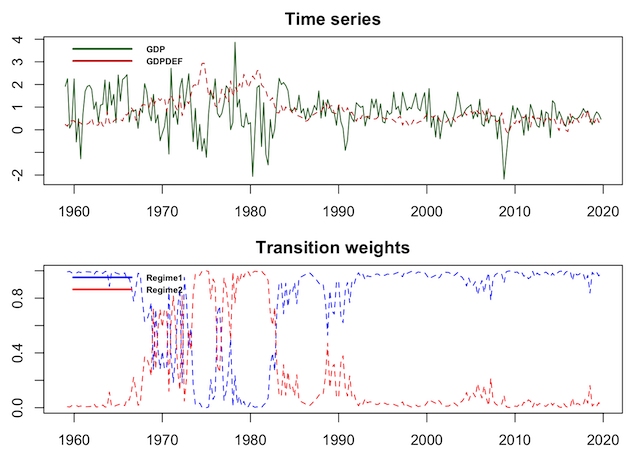
\includegraphics{figures/seriesplot.png}
  \caption{The figure produced by the command \code{plot(fit12)}. On the top, a quarterly series consisting of two U.S. variables: the percentage change of real GDP and the percentage change of GDP implicit price deflator, covering the period from 1959Q1 to 2019Q4. On the bottom, the estimated transition weights of the STVAR model \code{fit12gs} fitted the series.}
\label{fig:seriesplot}\end{figure}

It is also sometimes interesting to examine the time series of (one-step) conditional means of the process along with the time series the model was fitted to. This can be done conveniently with the function by setting the argument \code{plot_type="cond_mean"} in the plot method. This plot depicts the contribution of each regime to the conditional mean of the process and how close the conditional mean is to the observed series in each point of time.

The variable metric algorithm employed in the final estimation does not necessarily stop at a local maximum point. The algorithm might also stop at a saddle point or near a local maximum, when the algorithm is not able to increase the log-likelihood, or at any point, when the maximum number of iterations has been reached. In the latter case, the estimation function throws a warning, but saddle points and inaccurate estimates need to be detected by the researcher.

It is well known that in a local maximum point, the gradient of the log-likelihood function is zero, and the eigenvalues of the Hessian matrix are all negative. In a local minimum, the eigenvalues of the Hessian matrix are all positive, whereas in a saddle point, some of them are positive and some negative. Nearly numerically singular Hessian matrices occur when the surface of the log-likelihood function is very flat about the estimate in some directions. This particularly happens when the transition weights $\alpha_{m,t}$ are estimated close to zero for all $t=1,...,T$ for some regime $m$.

\pkg{sstvars} provides several functions for evaluating whether the estimate is a local maximum point. The function \code{get_foc} returns the (numerically approximated) gradient of the log-likelihood function evaluated at the estimate, and the function \code{get_soc} returns eigenvalues of the (numerically approximated) Hessian matrix of the log-likelihood function evaluated at the estimate. The numerical derivatives are calculated using a central difference approximation
\begin{equation}
\frac{\partial L(\boldsymbol{\theta})}{\partial \theta_i} \approx \frac{f(\boldsymbol{\theta} + \boldsymbol{h}^{(i)}) - f(\boldsymbol{\theta} - \boldsymbol{h}^{(i)})}{2h}, \ \ h>0,
\end{equation}
where $\theta_i$ is the $i$th element of $\boldsymbol{\theta}$ and $\boldsymbol{h}^{(i)}=(0,...,0,h,0,...,0)$
contains $h$ as its $i$th element. By default, the difference $h=6\cdot 10^{-6}$ is used.

For example, the following code calculates the first order condition for the G-StMVAR model \code{fit12}:
%
\begin{CodeChunk}
\begin{CodeInput}
R> get_foc(fit12)
\end{CodeInput}
\begin{CodeOutput}
 [1]  4.262025e-04  4.048578e-04  1.281037e-04 -5.780028e-04
 [5]  3.221411e-04  1.776783e-04  2.645895e-04 -3.844178e-04
 [9] -2.174971e-05  1.380419e-04  1.664494e-04 -8.551879e-04
[13]  1.246268e-04 -3.826628e-04 -2.131233e-03 -2.536638e-06
[17]  1.432667e-04  1.818326e-04  3.602239e-04  1.000681e-05
[21] -3.700270e-05
\end{CodeOutput}
\end{CodeChunk}
%
and the following code calculates the second order condition:
%
\begin{CodeChunk}
\begin{CodeInput}
R> get_soc(fit12)
\end{CodeInput}
\begin{CodeOutput}
 [1] -1.494320e-01 -2.682544e-01 -1.047386e+00 -6.177532e+00
 [5] -9.934297e+00 -1.654975e+01 -5.366908e+01 -7.191557e+01
 [9] -1.215715e+02 -1.673756e+02 -1.859815e+02 -2.718937e+02
[13] -3.775367e+02 -3.834231e+02 -6.567316e+02 -9.911009e+02
[17] -1.227186e+03 -1.377650e+03 -8.775102e+03 -9.731932e+03
[21] -3.895717e+04
\end{CodeOutput}
\end{CodeChunk}
%
All eigenvalues of the Hessian matrix are negative, which points to a local maximum, and the gradient of the log-likelihood function is close to zero. The gradient is not exactly zero, because it is based on a numerical approximation. It is also possible that the estimate is inaccurate, because it is based on approximative numerical estimation, and the estimates are therefore not expected to be exactly accurate. Whether the estimate is a local maximum point with accuracy that is reasonable enough, can be evaluated by plotting the graphs of the profile log-likelihood functions about the estimate. In \pkg{sstvars}, this can be done conveniently with the function \code{profile_logliks}.

The exemplify, the following command plots the graphs of profile log-likelihood functions of the estimated G-StMVAR model \code{fit12}:
%
\begin{CodeChunk}
\begin{CodeInput}
R> profile_logliks(fit12, scale=0.02, precision=200)
\end{CodeInput}
\end{CodeChunk}
%
The resulting plot is presented in Figure~\ref{fig:proflogliks}.

\begin{figure}[t]
  \centering
  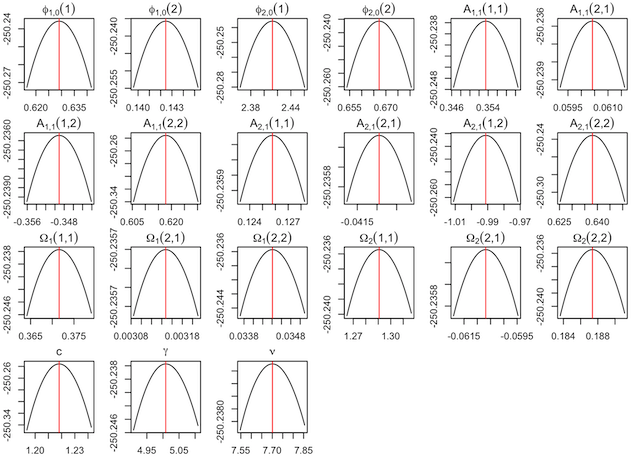
\includegraphics{figures/profilelogliks.png}
  \caption{The figure produced by the command \code{profile\_logliks(fit12, scale=0.02, precision=200)}. The graphs of the profile log-likelihood functions of the logistic Student's $t$ STVAR model drawn about the estimate. The red vertical lines denote the estimate.}
\label{fig:proflogliks}
\end{figure}

The output shows that the estimate's accuracy is reasonable, as changing any individual parameter value marginally would not increase the log-likelihood much. The argument \code{scale} can be adjusted to shorten or lengthen the interval shown in the horizontal axis. If one zooms in enough by setting \code{scale} to a very small number, it can be seen that the estimate is not exactly at the local maximum, but it is so close that moving there would not increase the log-likelihood notably. The argument \code{precision} can be adjusted to increase the number of points the graph is based on. For faster plotting, it can be decreased, and for more precision, it can be increased. The argument \code{which_pars} is used to specify the parameters whose profile log-likelihood functions should be plotted. This argument is particularly useful when creating as many plots as there are parameters in the model to a single figure would cause the individual plots to be very small. In such a case, profile log-likelihood functions for subsets of the parameters can be plotted separately by specifying this argument accordingly.

We have discussed tools that can be utilized to evaluate whether the found estimate is a local maximum with a reasonable accuracy. It is, however, more difficult to establish that the estimate is the global maximum. With \pkg{sstvars}, the best way to increase the reliability that the found estimate is the global maximum (among the appropriate solutions), is to run more estimation rounds by adjusting the argument \code{nrounds} of the estimation function \code{fitSTVAR}.

If the model is very large, a very large number of estimation rounds may be required to find the global maximum. If there are two regimes in the model, $p$ is reasonable, and the dimension of the time series at most four, the required number of estimation rounds typically varies from several hundred to several thousand depending on the model and the data. In the simpler models, less estimation rounds are required. In the larger models, and in particular if $M>2$ or $d>4$, a significantly large number of estimation rounds may be required obtain the MLE. Another thing that makes the estimation more challenging, are exotic parameter constraints that do not reduce the dimension of the parameter much. Constraints that greatly reduce complexity of the parameter space (such as constraining the autoregressive matrices to be identical in all regimes\footnote{Models constrained in this way can often be reliably estimated with a reasonable number of estimation rounds even when $M>2$}), on the other hand, make the estimation easier, and reliable estimation of such models thereby require less estimation rounds. Constrained estimation is discussed in Section~\ref{sec:examp_const}.

\subsection{Estimation of structural STVAR models}\label{sec:estim_structural}
As explained, \pkg{sstvars} currently supports three types of structural models: structural models identified recursively by the lower triangular Cholesky decomposition, structural models identified by conditional heteroskedasticity, and structural models identified by non-Gaussianity. In either case, the structural models are estimated with the function \code{fitSSTVAR} based on preliminary estimates from a reduced form model. If the structural model is not overidentifying, which is always the case for recursively identified models, model identified by non-Gaussianity, as well as for models identified by heteroskedasticity when there are two regimes and further constraints are not imposed on the impact matrix, there is no need for estimation but at most for a reparametrization of the model. In any case, the \code{fitSSTVAR} constructs the structural model appropriately.

To exemplify, we first create a recursively identified structural model based on the reduced form model \code{fit12} by setting the argument \code{identification="recursive"}. Then, we will study an example of a structural model identified by heteroskedasticity. The following code builds the recursively identified model:
\begin{CodeChunk}
\begin{CodeInput}
R> fit12rec <- fitSSTVAR(fit12, identification="recursive")
\end{CodeInput}
\end{CodeChunk}
Since the parametrization did not change nor was any estimation required, \code{fit12rec} is essentially the reduced form model \code{fit12} with has the property that can be used as a structural model in structural analysis such as for estimating the generalized impulse response functions.

The following code creates a structural model identified by heteroskedasticity based on the reduced form model \code{fit12} and then prints it:
\begin{CodeChunk}
\begin{CodeInput}
R> fit12het <- fitSSTVAR(fit12, identification="heteroskedasticity")
R> print(fit12het)
\end{CodeInput}
\begin{CodeOutput}
logistic Student STVAR model, identified by heteroskedasticity, no AR_constraints,
no mean_constraints, no B_constraints,
  p = 1, M = 2, d = 2, #parameters = 21, #observations = 243 x 2
  Switching variable: GDPDEF with lag 1.

Regime 1
Degrees of freedom: 7.70 (for all regimes)
Regime means: 0.71, 0.49

   Y     phi0          A1                  Omega        1/2
1 y1 = [ 0.63 ] + [  0.35 -0.35 ] y1.1 + [  0.37 0.00 ]     eps1
2 y2   [ 0.14 ]   [  0.06  0.62 ] y2.1   [  0.00 0.03 ]     eps2

Regime 2
Weight params: 1.22 (location), 5.01 (scale)
Regime means: 0.77, 1.76

   Y     phi0          A1                  Omega         1/2
1 y1 = [ 2.41 ] + [  0.13 -0.99 ] y1.1 + [  1.29 -0.06 ]     eps1
2 y2   [ 0.67 ]   [ -0.04  0.64 ] y2.1   [ -0.06  0.19 ]     eps2

Structural parameters:
        W             lamb2
1 [  0.17  0.59 ]   [  5.67 ]
2 [ -0.18  0.06 ] , [  3.29 ]

The impact matrix is subject to 0 zero constraints and 0 sign constraints.
\end{CodeOutput}
\end{CodeChunk}
%
Since the structural model identified by heteroskedasticity is not overidentified, no estimation was performed but merely a reparametrization. The estimates for the structural parameters $W$ and $\lambda_2,...,\lambda_M$ are presented at the bottom of the printout.

If the structural model is identified by heteroskedasticity or non-Gaussianity, additional restrictions can be imposed on the impact matrix by setting them in the argument \code{B_constraints}. A structural model identified by heteroskedasticity is overidentifying also when there are more than two regimes in the model, as then the matrix decomposition employed in the identification does not always exist. In either case, the structural model needs be estimated, which is performed in \code{sstvars} based on preliminary estimates obtained either from a reduced form model or from a structural model. The estimation is performed with the function \code{fitSSTVAR}, which implements a two-phase estimation procedure in which a robust estimation method is used in the first phase and a variable algorithm in the second phase. The default option for the robust method is Nelder-Mead algorithm implemented by \cite{R} in the function \code{optim} of the package \code{stats}.

It is important to note that if the initial estimates are far from the ML estimate of the overidentified model, the resulting solution is likely local only due to the high multimodality of the log-likelihood function. However, it is not often very appealing to impose overidentified constraints that far from the unrestricted estimates in the first place. But in any case, since the estimation may be unrealiable if the restricted ML estimate is far from the unrestricted ML estimate, we recommend using our package to estimate only such overidentifying structural models in which the unrestricted estimate is close to satisfying the imposed constraints.

The exemplify, we estimate a structural model identified by heteroskedasticity based on the structural model \code{fit12het} by setting the argument \code{identification="heteroskedasticity"} and imposing the constraint that the second element of the second column of the impact matrix is zero (the above estimates of $W$ show that the corresponding unrestricted estimate is close to zero). The zero constraint is imposed by setting the argument \code{B_constraints} as matrix such that the second element of the second column is zero and all other elements are \code{NA}. Sign constraints can be set similarly by setting the corresponding elements to \code{1} or \code{-1} (or any other strictly positive of negative value). The following code estimates the model:
\begin{CodeChunk}
\begin{CodeInput}
R> fit12hetb <- fitSSTVAR(fit12, identification="heteroskedasticity",
+    B_constraints=matrix(c(NA, NA, NA, 0), nrow=2))
R> print(fit12het)
\end{CodeInput}
\begin{CodeOutput}
The log-likelihood of the supplied model:    -250.236
Constrained log-likelihood prior estimation: -260.164
The log-likelihood after robust estimation:  -250.556
The log-likelihood after final estimation:   -250.486
\end{CodeOutput}
\end{CodeChunk}
The log-likelihoods of the original model, the initial estimates of the constrained model, the estimates after the robust estimation, and the final estimates are printed. If the log-likelihood of after final estimation is bad compared to the log-likelihood of the original model, the estimation is likely unreliable. The command \code{print(fit12hetb)} prints the estimated overidentified model (we ommit the printout for brevity).

After creating a structural model identified by heteroskedasticity, the columns of $W$ can be reordered with the function \code{reorder_B_columns} which also reorders all $\lambda_{mi}$ accordingly (and hence the resulting model will coincide with the original reduced form model). Also, all signs of any column of $W$ can be swapped with the function \code{swap_B_signs}.

\subsection{Constrained estimation}\label{sec:examp_const}
\pkg{sstvars} supports constrained ML estimation of the STVAR models, including several types of constraints. Linear constraints can be imposed on the autoregressive matrices (argument \code{AR_constraints}), unconditional means of the regimes can be constrained equal across (groups of) regimes (argument \code{mean_constraints}), and weight function parameters can be constrained to a fixed value or linear constraints can be impose on them (argument \code{weight_constraints}). Following sections give examples of constrained estimation imposing some of these constraints.

\subsubsection{Linear constraints on the autoregressive parameters}
Imposing linear constraints on the autoregressive parameters of a STVAR model is straightforward in \pkg{sstvars}. The constraints are expressed in a somewhat general form which allows to impose a wide class of constraints but one needs to take the time to construct the constraint matrix carefully for each particular case.

We consider constraints of form
\begin{align}
& (\boldsymbol{\phi}_1,...,\boldsymbol{\phi}_M) = \boldsymbol{C}\boldsymbol{\psi},\\
& \boldsymbol{\phi}_m=(vec(A_{m,1}),...,vec(A_{m,p}))\enspace (pd^2x1), \enspace m=1,...,M,
\end{align}
where $\boldsymbol{C}$ is known $(Mpd^2xq)$ constraint matrix (of full column rank) and $\boldsymbol{\psi}$ is unknown $(qx1)$ parameter vector.

To give couple examples, consider the following two common uses of linear constraints: restricting the autoregressive matrices to be the equal across all regimes and constraining some of the AR parameters to zero.

\textbf{Restricting AR matrices to be the equal across the regimes}\\
To restrict the AR matrices to be equal across the regimes, we want $\boldsymbol{\phi}_m$ to be the same for all $m=1,...,M$. The parameter vector $\boldsymbol{\psi}$ $(qx1)$ then corresponds to any $\boldsymbol{\phi}_m=\boldsymbol{\phi}$, and therefore $q=pd^2$. For the constraint matrix we choose
\begin{equation}
\boldsymbol{C} = [I_{pd^2}:\cdots:I_{pd^2}]' \enspace (Mpd^2xpd^2),
\end{equation}
that is, $M$ pieces of $(pd^2xpd^2)$ diagonal matrices stacked on top of each other, because then
\begin{equation}
\boldsymbol{C}\boldsymbol{\psi}=(\boldsymbol{\psi},...,\boldsymbol{\psi})=(\boldsymbol{\phi},...,\boldsymbol{\phi}).
\end{equation}
For instance, if there are two regimes in the model, the appropriate constraint matrix then created as
%
\begin{CodeChunk}
\begin{CodeInput}
R> p <- 1 # The autoregressive order of the model
R> d <- 2 # Whatever the dimension of the time series is
R> I_pd2 <- diag(p*d^2) # The appropriate diagonal matrix
R> (C1 <- rbind(I_pd2, I_pd2)) # Stack them on top of each other
\end{CodeInput}
\begin{CodeOutput}
     [,1] [,2] [,3] [,4]
[1,]    1    0    0    0
[2,]    0    1    0    0
[3,]    0    0    1    0
[4,]    0    0    0    1
[5,]    1    0    0    0
[6,]    0    1    0    0
[7,]    0    0    1    0
[8,]    0    0    0    1
\end{CodeOutput}
\end{CodeChunk}
%
The command
\begin{CodeChunk}
\begin{CodeInput}
R> fit12c1 <- fitSTVAR(gdpdef, p=1, M=2, weight_function="logistic",
+    weightfun_pars=c(2, 1), cond_dist="Student", AR_constraints=C1)
\end{CodeInput}
\end{CodeChunk}
would then estimate a logistic Student's $t$ STVAR($1,2$) model with first lag of the second variable as the switching variable such that the AR matrices constrained to be the equal in both regimes. We omit the output for brevity. In practice, you might want to adjust the number of CPU cores used (\code{ncores}), the of estimation rounds (\code{nrounds}), and set seeds (\code{seeds}).

\textbf{Restricting AR parameters to be the same for all regimes and constraining non-diagonal elements of coefficient matrices to be zero}\\
The previous example shows how to restrict the AR parameters to be the same for all regimes, but say we also want to constrain the non-diagonal elements of coefficient matrices $A_{m,i}$ $(m=1,...,M, i=1,...,p)$ to be zero. We have the constrained parameter $\boldsymbol{\psi}$ $(qx1)$ representing the unconstrained parameters $(\boldsymbol{\phi}_1,...,\boldsymbol{\phi}_M)$, where the restrictions imply $\boldsymbol{\phi}_m=\boldsymbol{\phi}=(vec(A_1),...,vec(A_p))$ $(pd^2x1)$ and the elements of $vec(A_i)$ $(i=1,...,p)$ corresponding to the diagonal are zero.

For illustrative purposes, let's consider a STVAR model with autoregressive degree $p=2$, number of regimes $M=2$, and number of time series in the system $d=2$. Then we have
\begin{align}
\boldsymbol{\phi}&=(A_1(1,1),0,0,A_1(2,2),A_2(1,1),0,0,A_2(2,2)) \enspace (8x1) \enspace \text{and}\\
\boldsymbol{\psi}&=(A_1(1,1),A_1(2,2),A_2(1,1),A_2(2,2)) \enspace (4x1),
\end{align}
where $A_l(i,j)$ is the $ij$th elements of $A_l$. By a direct calculation, we can see that choosing the constraint matrix
\begin{equation}
\boldsymbol{C}=\left[{\begin{array}{c}
   \boldsymbol{\tilde{c}} \\
   \boldsymbol{\tilde{c}} \\
  \end{array}}\right]
\enspace (Mpd^2x4),
\enspace
\end{equation}
where
\begin{equation}
\boldsymbol{\tilde{c}}=\left[{\begin{array}{cccc}
   1 & 0 & 0 & 0 \\
   0 & 0 & 0 & 0 \\
   0 & 0 & 0 & 0 \\
   0 & 1 & 0 & 0 \\
   0 & 0 & 1 & 0 \\
   0 & 0 & 0 & 0 \\
   0 & 0 & 0 & 0 \\
   0 & 0 & 0 & 1 \\
  \end{array}}\right]
\enspace (pd^2x4)
\end{equation}
satisfies $\boldsymbol{C}\boldsymbol{\psi}=(\boldsymbol{\phi},...,\boldsymbol{\phi}).$

The above constraint matrix can be created as
%
\begin{CodeChunk}
\begin{CodeInput}
R> c_tilde <- matrix(0, nrow=2*2^2, ncol=4)
R> c_tilde[c(1, 12, 21, 32)] <- 1
R> C2 <- rbind(c_tilde, c_tilde)
R> C2
\end{CodeInput}
\begin{CodeOutput}
      [,1] [,2] [,3] [,4]
 [1,]    1    0    0    0
 [2,]    0    0    0    0
 [3,]    0    0    0    0
 [4,]    0    1    0    0
 [5,]    0    0    1    0
 [6,]    0    0    0    0
 [7,]    0    0    0    0
 [8,]    0    0    0    1
 [9,]    1    0    0    0
[10,]    0    0    0    0
[11,]    0    0    0    0
[12,]    0    1    0    0
[13,]    0    0    1    0
[14,]    0    0    0    0
[15,]    0    0    0    0
[16,]    0    0    0    1
\end{CodeOutput}
\end{CodeChunk}
%
The command
\begin{CodeChunk}
\begin{CodeInput}
R> fit12c2 <- fitSTVAR(gdpdef, p=2, M=2, weight_function="logistic",
+    weightfun_pars=c(2, 1), cond_dist="Student", AR_constraints=C2)
\end{CodeInput}
\end{CodeChunk}
would then estimate a logistic Student's $t$ STVAR($1,2$) model with first lag of the second variable as the switching variable such that the AR matrices are constrained to be the equal in both regimes and the off-diagonal elements are restricted to zero. Again, we omit the output for brevity (and you may want to adjust the arguments \code{nrounds}, \code{ncores}, and \code{seeds} when estimating the model in practice).


\subsubsection{Constraining the unconditional means of some regimes to be equal}
In addition to constraining the autoregressive parameters, \pkg{sstvars} allows to constrain the unconditional means of some regimes to be the equal. This feature is, however, only available for models that are parametrized with the unconditional means instead of intercepts (because some of the estimation is always done with mean-parametrization and one cannot generally swap the parametrization when constraints are imposed on means/intercepts). With the mean-parametrization employed (by setting \code{parametrization="mean"}), one may define groups of regimes that have the same mean parameters using the argument \code{mean_constraints}. For instance, with three regime model $(M=3)$ the argument \code{mean_constraints=list(c(1, 3), 2)} sets the unconditional means of the first and third regimes to be the same while allows the second regime to have different mean.

One can also combine linear constraints on the AR parameters with constraining some of the means to be the same. This allows, for instance, to estimate a model in which only the covariance matrix varies in time. To exemplify, the following code estimates a Student's $t$ logistic STVAR($p=1, M=2$) model such that the unconditional means and autoregression matrices are constrained be the same in both regimes. The resulting model thereby has time-varying covariance matrix but otherwise it is linear.
%
\begin{CodeChunk}
\begin{CodeInput}
R> fit12c3 <- fitSTVAR(gdpdef, p=1, M=2, weight_function="logistic",
+    weightfun_pars=c(2, 1), cond_dist="Student", AR_constraints=C1,
+    mean_constraints=list(1:2), parametrization="mean")
\end{CodeInput}
\end{CodeChunk}
%
The output is omitted for brevity.

\subsubsection{Constraining weight functions parameters}
It is also possible to constrain the weight functions parameters $\alpha$ (e.g., the location and scale parameters for logistic models). \pkg{sstvars} accommodates two types of alternative constraints on the weight function parameters: linear constraints and fixed values. Note that weights constraints are not available for models with exogenous weights, as they do not contain any weight function parameters.

\textbf{Linear constraints}\\
Linear constraints on the weight function parameters are of the form
\begin{equation}
\alpha = R\xi + r,
\end{equation}
where $\alpha$ ($a \times 1$) contains the weight funtion parameters, $R$ is a known $(a \times l)$ constraint matrix of full column rank, $r$ is a known $(a \times 1)$ constant, and $\xi$ is an unknown $(l \times 1)$ parameter. The constraint matrix $R$ and the constant $r$ are set in the argument \code{weight_constraints} as a list of two elements, $R$ in the first element and $r$ in the second element. The number of unknown parameters $l$ is the number of columns of $R$. For instance, the following argument imposes constraints for the scale and location parameters of a logistic STVAR model (in which $\alpha = (c,\gamma)$) such that the location parameter is the scale parameter divided by two plus $0.3$: \code{weight_constraints=list(R=matrix(c(0.5, 1), nrow=2), r=c(0.3, 0))}.

\textbf{Fixed values}\\
Imposing the weight function parameters to be known fixed values is very straightforward. In this case, the argument \code{weight_constraints} should still be a list including the elements $R$ and $r$, but the former is set to zero, $R=0$, and the latter is set to the desired fixed values. For instance the following argument imposes constraints for the location and location parameters of a logistic STVAR model (in which $\alpha = (c,\gamma)$) such that the location parameter is $0.3$ and the scale parameter is $0.5$: \code{weight_constraints=list(R=0, r=c(0.3, 0.5)}.

\subsection{Testing parameter constraints}\label{sec:testconst}
One way to asses the validity of the imposed constraints is to compare the values of information criteria of the constrained and unconstrained models. \pkg{sstvars}, however, also provides functions for testing the constraints with the likelihood ratio test, Wald test, and Rao's test, whose applicability requires that the ML estimator of the STVAR model has the conventional asymptotic distribution. As noted before, this is a mere assumption, but given the process is ergodic stationary, there is no particular reason to believe that the standard asymptotic results would not hold. For a discussion on the tests, see \citet{Buse:1982} and the references therein, for example.

The likelihood ratio test considers the null hypothesis that the true parameter value $\boldsymbol{\theta}_0$ satisfies some constraints imposed on these parameters (such that the constrained parameter space is a subset of the parameter space, which is presented in Assumption~\ref{as:mle}). Denoting by $\hat{L}_U$ and $\hat{L}_C$ the (maximized) log-likelihoods based on the unconstrained and constrained ML estimates, respectively, the test statistic takes the form
\begin{equation}
LR=2(\hat{L}_U - \hat{L}_C).
\end{equation}
Under the null, the test statistic is asymptotically $\chi^2$-distributed with the degrees of freedom given by the difference in the dimensions of the unconstrained and constrained parameter spaces. With \pkg{sstvars}, the likelihood ratio test can be calculated with the function \code{LR_test}, which takes the unconstrained model (a class \code{'stvar'} object) as its first argument and the constrained model as the second argument.

\pkg{sstvars} implements the Wald test of the null hypothesis
\begin{equation}
A\boldsymbol{\theta}_0 = c,
\end{equation}
where $A$ is a $(k \times d)$ matrix with full row rank, $c$ is a $(k \times 1)$ vector, $\boldsymbol{\theta}_0$ is the true parameter value, $d$ is the dimension of the parameter space, and $k$ is the number of constraints. The Wald test statistic takes the form
\begin{equation}
W = (A\hat{\boldsymbol{\theta}} - c)' [A\mathcal{J}(\hat{\boldsymbol{\theta}})^{-1}A']^{-1}(A\hat{\boldsymbol{\theta}} - c),
\end{equation}
where $\mathcal{J}(\hat{\boldsymbol{\theta}})$ is the observed information matrix evaluated at the ML estimate $\hat{\boldsymbol{\theta}}$. Under the null, the test statistic is asymptotically $\chi^2$-distributed with $k$ degrees of freedom (which is the difference in dimensions of the constrained and unconstrained parameter spaces). With \pkg{sstvars}, the Wald test can be calculated with function \code{Wald_test}, which takes the estimated unconstrained model (as a class \code{'stvar'} object) as the first argument, the matrix $A$ as the second argument, and the vector $c$ as the third argument.

Finally, Rao's test is implemented to the function \code{Rao_test}. See the function documentation on how to use it.

\section{Residual based model diagnostics}\label{sec:res}
\pkg{sstvars} employs residual based diagnostics for assessing the adequacy of the fitted model. Conventional graphical diagnostics can be examined with function \code{diagnostic_plot}, which plots the residual time series, auto- and crosscorrelation functions of the residuals, auto- and crosscorrelation functions of the squared residuals, and normal quantile-quantile plots as well as histograms of the residuals. The plots can be created for both unstandardized residuals or for standardized residuals by adjusting the argument \code{standardize} to \code{FALSE} or \code{TRUE} according. Using unstandardized residuals is advisable when checking for remaining autocorrelation. But standardized residuals should be used to check for remaining conditional heteroskedasticity and to check the model's adequacy to capture the marginal distribution of the series, because the STVAR models are conditionally heteroskedastic and the unstandardized residuals do not take into account the time-varying conditional covariance matrix.

Remaining autocorrelation in the residuals can also be tested with the (adjusted) Portmanteau test, which is implemented to the function \code{Portmantau_test}. The test can also be applied to standardized squared residuals to test for remaining conditional heteroskedasticity by setting the argument \code{which_test="het.sked"}. The number of lags that should be taken into account in the test is set with the argument \code{nlags}.


\section{Impulse response analysis}\label{sec:impulseresponse}

\subsection{Generalized impulse response function}
The expected effects of the structural shocks in the structural STVAR models generally depend on the initial values as well as on the sign and size of the shock, which makes the conventional way of calculating impulse responses unsuitable \citep[see, e.g.,][Chapter~4]{Kilian+Lutkepohl:2017}. Therefore, we  consider the generalized impulse response function (GIRF) \citep{Koop+Pesaran+Potter:1996} defined as
\begin{equation}\label{eq:girf}
\text{GIRF}(n,\delta_j,\mathcal{F}_{t-1}) = \text{E}[y_{t+n}|\delta_j,\mathcal{F}_{t-1}] - \text{E}[y_{t+n}|\mathcal{F}_{t-1}],
\end{equation}
where $n$ is the chosen horizon, $\mathcal{F}_{t-1}=\sigma\lbrace y_{t-j},j>0\rbrace$ as before, the first term on the right side is the expected realization of the process at time $t+n$ conditionally on a structural shock of sign and size $\delta_j \in\mathbb{R}$ in the $j$th element of $e_t$ at time $t$ and the previous observations, and the second term on the right side is the expected realization of the process conditionally on the previous observations only. GIRF thus expresses the expected difference in the future outcomes when the specific structural shock hits the system at time $t$ as opposed to all shocks being random.

Due to the $p$-step Markov property of the implemented STVAR models, conditioning on (the $\sigma$-algebra generated by) the $p$ previous observations $\boldsymbol{y}_{t-1}\equiv(y_{t-1},...,y_{t-p})$ is effectively the same as conditioning on $\mathcal{F}_{t-1}$ at the time $t$ and later. The initial values (or history) $\boldsymbol{y}_{t-1}$ can be either fixed or random, but with random history the GIRF becomes a random vector, however. Using fixed $\boldsymbol{y}_{t-1}$ makes sense when one is interested in the effects of the shock in a particular point of time. Alternatively, one can estimate GIRFs conditional on the initial values being from a specific regime, in which case $\boldsymbol{y}_{t-1}$ should generated from the regime of interest.

In practice, the GIRF and its distributional properties can be approximated with a Monte Carlo algorithm that generates independent realizations of the process and then takes the sample mean for point estimate. If $\boldsymbol{y}_{t-1}$ is random and follows the distribution $G$, the GIRF should be estimated for different values of $\boldsymbol{y}_{t-1}$ generated from $G$, and then the sample mean and sample quantiles can be taken to obtain the point estimate and confidence intervals. The algorithm implemented in \pkg{sstvars} is presented in \cite{Lanne+Virolainen:2024}.

Because the STVAR models allow to associate specific features or economic interpretations for different regimes, and because shifts in the regime are the source of asymmetries in the impulse responses, it might be interesting to also examine the effects of a structural shock to the transition weights $\alpha_{m,t}$, $m=1,...,M$. We then consider the related GIRFs $E[\alpha_{m,t+n}|\delta_j,\boldsymbol{y}_{t-1}] - E[\alpha_{m,t+n}|\boldsymbol{y}_{t-1}]$ for which point estimates and confidence intervals can be constructed similarly to (\ref{eq:girf}).

In \pkg{sstvars}, the GIRF can be estimated with the function \code{GIRF} which should be supplied with the estimated STVAR model or a STVAR model built with hand-specified parameter values using the function \code{STVAR}. Structural models can be created based on a reduced form model with the function \code{fitSSTVAR}. The sign and size of the structural shock can be set with the argument \code{shock_size}. If not specified, a positive shock with the size of one standard deviation is used; that is, the size is one. Among other arguments, the function may also be supplied with the argument \code{init_regime} which specifies from which regime the initial values are generated from. Alternatively, one may specify fixed initial values with the argument \code{init_values}. Note that the confidence intervals (whose confidence level can be specified with the argument \code{ci}) reflect uncertainty about the initial value only and not about the parameter estimates.

Due to the nonlinear nature of the model, GIRFs estimated from different starting values, or with different sign or magnitude of the shock, generally move the variables differently. Sometimes it is, however, of interest to scale the impulse responses so that they correspond to instantaneous movement of some specific sign and size of some specific variable. In \pkg{sstvars}, this is most conveniently achieved with the arguments \code{scale}. The argument \code{scale} can be specified in order to scale the GIRFs to some of the shocks so that they correspond to a specific sign and size of instantaneous response of some specific variable. Alternatively, the GIRFs can be scaled to correspond to a specific peak response of some variable by setting \code{scale_type="peak"}. For a single shock, the argument \code{scale} should a length three vector where the shock of interest is given in the first element (an integer in $1,...,d$), the variable according to which the GIRFs should be scaled in the second element (an integer in $1,...,d$), and the sign and size of the given variable's instantaneous response in the third element (a non-zero real number). If the GIRFs of multiple shocks should be scaled, provide a matrix which has one column for each of the shocks with the columns being the length three vectors described above. Note that if you scale the GIRFs, the scaled GIRFs of transition weights can be outside the interval from zero to one.

Because estimating the GIRF and their confidence intervals is computationally demanding, parallel computing is taken use of to shorten the estimation time. The number of CPU cores used can be set with the argument \code{ncores}. The objects returned by the \code{GIRF} function have their own \code{plot} and \code{print} methods. Also, cumulative impulse responses of the specified variables can be obtained directly by specifying the argument \code{which_cumulative}.

\subsection{Generalized forecast error variance decomposition}
Similarly to the conventional impulse response functions are unsuitable for impulse response analysis (due to their inability to capture asymmetries the effects of the shocks), the conventional forecast error variance decomposition is unsuitable for tracking the contribution of each shock to the variance of the forecast errors. We consider the generalized forecast error variance decomposition (GFEVD) \citep{Lanne+Nyberg:2016}  that is defined for variable $i$, shock $j$, and horizon $h$ as
\begin{equation}
\text{GFEVD}(j,y_{it}, \delta_j,\mathcal{F}_{t-1}) = \frac{\sum_{l=0}^h\text{GIRF}(l,\delta_j,\mathcal{F}_{t-1})_i^2}{\sum_{k=1}^d\sum_{l=0}^h\text{GIRF}(l,\delta_k,\mathcal{F}_{t-1})_i^2},
\end{equation}
where $h$ is the chosen horizon and $\text{GIRF}(l,\delta_j,\mathcal{F}_{t-1})_i$ is the $i$th element of the related GIRF (see also the notation described for GIRF in the previous section). That is, the GFEVD is otherwise similar to the conventional forecast error variance decomposition but with GIRFs in the place of conventional impulse response functions. Because the GFEVDs sum to unity (for each variable), they can be interpreted in a similar manner to the conventional FEVD.

In \pkg{sstvars}, the GFEVD can be estimated with the function \code{GFEVD}. As with the GIRF, the GFEVD is dependent on the initial values. The type of the initial values is set with the argument \code{initval_type}, and there are three options:
\begin{enumerate}
\item \code{"data"} which estimates the GIRFs for all possible length $p$ histories in the data and then the GIRFs in the GFEVD are obtained as the sample mean over those GIRFs.
\item \code{"random"} which generates the initial values from one of the specific regimes, specified by the argument \code{init_regimes}. The GIRFs in the GFEVD are obtained as the sample mean over the GIRFs estimated for the different random initial values.
\item \code{"fixed"} which estimates the GIRFs for a single fixed initial value that is set with the argument \code{init_values}.
\end{enumerate}
The shock size is the same for all scalar components of the structural shock and it can be adjusted with the argument \code{shock_size}. If the GIRFs for some variables should be cumulative before calculating the GFEVD, specify them with the argument \code{which_cumulative}. Finally, note that the GFEVD objects have their own plot and print methods.

\code{sstvars} also implements a special feature in which for every possible length p history in the data, the GFEVD is estimated for a shock that has the sign and size of the corresponding structural shock recovered from the fitted model. This can be done by setting the argument \code{use_data_shocks=TRUE}. The GFEVD is then calculated as the average of the GFEVDs obtained from the GIRFs estimated for the data shocks. The plot and print methods can be used as usual for this GFEVD. However, this feature also estimates the contribution of each shock to the variance of the forecast errors at various horizons in specific historical points of time. This can be done by using the plot method with the argument \code{data_shock_pars}. Note that the arguments \code{shock_size}, \code{initval_type}, and \code{init_regime} are ignored if \code{use_data_shocks == TRUE}.

\subsection{Linear impulse response functions}
It is also possible to calculate linear impulse response functions (IRF) based on a specific regime of the estimated model by using the function \code{linear_IRF}. If the autoregressive dynamics of the model are linear (i.e., either $M=1$ or mean and AR parameters are constrained identical across the regimes), confidence bounds can be estimated based on a type of a fixed-design wild residual bootstrap method. \code{sstvars} implements the method proposed \cite{Herwartz+Lutkepohl:2014}.

\section{Building a STVAR model with specific parameter values}\label{sec:STVAR}
The function \code{STVAR} facilitates building STVAR models without estimation, for instance, in order to simulate observations from a STVAR process with specific parameter values. The function should be supplied at least with the arguments \code{p}, \code{M}, and \code{d} specifying the autoregressive order, the number of regimes, and the dimension of the time series, respectively. The argument \code{params} should be used to specify the parameter values, whereas the weight function and weight function parameters are specified in the arguments \code{weight_function} and \code{weightfun_pars}, respectively, and the conditional distribution in the function \code{cond_dist}.

To exemplify, we build a reduced form Gaussian STVAR $p=1$, $M=1$, $d=2$ model with relative stationary densities as the transition weights. The model has intercept parametrization and parameter values $\varphi_{1,0}=(0, 1)$, $\varphi_{12,0}=(0, 2)$, $\text{vec}(A_{1,1}) = (0.2, 0.2, 0.2, -0.2)$, $\text{vec}(A_{1,1}) = (0.3, 0.3, 0.3, -0.3)$, $\text{vech}(\Omega_1) = (1, 0.1, 1)$, $\text{vech}(\Omega_2) = (4, 0.4, 4)$, and $\alpha_1$=0.6. After building the model, we use the \code{print} method to examine it:
%
\begin{CodeChunk}
\begin{CodeInput}
R> params122 <- c(0, 1, 0, 2, 0.2, 0.2, 0.2, -0.2, 0.3, 0.3, 0.3, -0.3, 1,
+    0.1, 1, 4, 0.4, 4, 0.6)
R> mod122 <- STVAR(p=1, M=2, d=2, params=params122,
+    weight_function="relative_dens")
R> mod122
\end{CodeInput}
\begin{CodeOutput}
relative_dens Gaussian STVAR model, reduced form model, no AR_constraints,
no mean_constraints,
  p = 1, M = 2, d = 2, #parameters = 19,

Regime 1
Weight param: 0.60
Regime means: 0.22, 0.87

   Y     phi0          A1                  Omega        1/2
1 y1 = [ 0.00 ] + [  0.20  0.20 ] y1.1 + [  1.00 0.10 ]     eps1
2 y2   [ 1.00 ]   [  0.20 -0.20 ] y2.1   [  0.10 1.00 ]     eps2

Regime 2
Weight param: 0.40
Regime means: 0.73, 1.71

   Y     phi0          A1                  Omega        1/2
1 y1 = [ 0.00 ] + [  0.30  0.30 ] y1.1 + [  4.00 0.40 ]     eps1
2 y2   [ 2.00 ]   [  0.30 -0.30 ] y2.1   [  0.40 4.00 ]     eps2
\end{CodeOutput}
\end{CodeChunk}
%

It is possible to include data in the models built with \code{STVAR} by either providing the data in the argument \code{data}. When the model is supplied with data, the transition weights and other data dependent statistics are calculated for the model as well.

\section{Simulation and forecasting}\label{sec:simufore}

\subsection{Simulation}\label{sec:simu}
\pkg{sstvars} implements the S3 method \code{simulate} for simulating observations from STVAR processes (see \code{?simulate.stvar}). The method requires the process to be given as a class \code{stvar} object, which are typically created either by estimating a model with the function \code{fitSTVAR} (or \code{fitSSTVAR}) or by specifying the parameter values by hand and building the model with the constructor function \code{STVAR}. The initial values required to simulate the first $p$ observations can be either set by hand (with the argument \code{init_values}) or drawn from (the stationary distribution of) some regime (with the argument \code{init_regime}). The argument \code{nsim} sets the length of the sample path to be simulated.

To give an example, the following code sets the random number generator seed to one and simulates $500$ observations long sample from the STVAR model built in Section~\ref{sec:STVAR}, drawing initial values from the first regime:
%
\begin{CodeChunk}
\begin{CodeInput}
R> mysim <- simulate(mod122, nsim=500, init_regime=1, seed=1)
\end{CodeInput}
\end{CodeChunk}
%
Our implementation of \code{simulate} returns a list containing the simulated sample path in \code{\$sample}, the mixture component that generated each observation in \code{\$component}, and the transition weights in \code{\$transition_weights}.

\subsection{Simulation based forecasting}
Deriving multiple-steps-ahead point predictions and prediction intervals analytically for the STVAR models is complicated, so \pkg{sstvars} employs the following simulation-based method. By using the last $p$ observations of the data up to the date of forecasting as initial values, a large number of sample paths for the future values of the process are simulated. Then, sample quantiles from the simulated sample paths are calculated to obtain prediction intervals, and the median or mean is used for point predictions. A similar procedure is also applied to forecast future values of the transition weights, which might be of interest because the researcher can often associate statistical characteristics or economic interpretations to the regimes.

Forecasting is most conveniently done with the \code{predict} method (see \code{?predict.stvar}). The available arguments include the number of steps ahead to be predicted (\code{nsteps}), the number sample paths the forecast is based on (\code{nsim}), possibly multiple confidence levels for prediction intervals (\code{pi}), prediction type (\code{pred_type}), and prediction interval type (\code{pi_type}). The prediction type can be either \code{median}, \code{mean} for the point forecast.

To exemplify, the following code forecasts the two-dimensional time-series of U.S. GDP and GDP deflator growth using the logistic Student's $t$ STVAR($1, 2$) model \code{fit12} estimated in Section~\ref{sec:example_estim}. The forecast is $10$ steps (quarters in this case) ahead, based on $10000$ Monte Carlo repetitions with the point forecast based on the mean of those repetitions. The prediction intervals are two-sided with confidence levels $0.95$ and $0.90$.
%
\begin{CodeChunk}
\begin{CodeInput}
R> mypred <- predict(fit12, nsteps=10, nsim=10000, pred_type="mean",
+    pi=c(0.95, 0.90))
\end{CodeInput}
\end{CodeChunk}
%
The results can be printed with the print method using the command \code{print(mypred)} or plotted with the plot method using the command \code{plot(mypred)}.


\begin{table}
\centering
\small
\begin{tabular}{llp{6.4cm}}
\hline
Related to     & Name                      & Description \\ \hline
Estimation     & \code{fitSTVAR}           & Estimate STVAR models.\\
               & \code{fitSSTVAR}          & Estimate or construct structural STVAR models.\\
               & \code{alt_stvar}          & Construct a STVAR model based on any estimation round.\\
               & \code{iterate_more}       & Run more iterations of the variable metric algorithm for a preliminary estimated STVAR model.\\
Estimates      & \code{print} (method)     & Print the estimates or their approximate standard errors.\\
               & \code{summary} (method)   & Detailed printout of the model.\\
               & \code{plot} (method)      & Plot the series with the fitted transition weights of the model.\\
               & \code{get_foc}            & Calculate numerically approximated gradient of the log-likelihood function evaluated at the estimate.\\
               & \code{get_soc}            & Calculate eigenvalues of numerically approximated Hessian of the log-likelihood function evaluated at the estimate.\\
               & \code{profile_logliks}    & Plot the graphs of the profile log-likelihood functions about the estimate.\\
Diagnostics    & \code{Portmanteau_test}   & Calculate the (adjusted) Portmanteau test.\\
               & \code{diagnostic_plot}    & Plot residual diagnostics (raw or standardized residuals).\\
Forecasting    & \code{predict} (method)   & Forecast future observations and transition weights of the process.\\
Simulation     & \code{simulate} (method)  & Simulate from a STVAR process.\\
Create model   & \code{STVAR}              & Construct a STVAR model based on given parameter values.\\
Hypothesis testing & \code{LR_test}        & Calculate likelihood ratio test.\\
               & \code{Wald_test}          & Calculate Wald test.\\
               & \code{Rao_test}           & Calculate Rao's test.\\
Impulse responses & \code{GIRF}    & Estimate generalized impulse response functions.\\
               & \code{GFEVD}              & Estimate generalized forecast error variance decomposition.\\
               & \code{linear_IRF}         & Estimate linear impulse response functions.\\
Other          & \code{bound_JSR} & Calculate bounds for the joint spectral radius of the companion form AR matrices of the regimes.\\
               & \code{swap_parametrization} & Swap between mean and intercept parametrizations \\
%               & \code{uncond_moments}     & Calculate unconditional moments of the regimes.\\
%               & \code{check_params}       & Check whether given parameter values satisfy our assumptions.\\
               & \code{swap_B_signs}       & Swap the signs of the columns of the impact matrix of models identified by heteroskedasticity. \\
               & \code{reorder_B_columns}  & Reorder the columns of the impact matrix of models identified by heteroskedasticity. \\
\hline
\end{tabular}
\caption{Some useful functions in \pkg{sstvars} sorted according to their usage. The note "method" in parentheses after the name of a function signifies that it is an S3 method for a class \code{stvar} object (often generated by the function \code{fitSTVAR}, \code{fitSSTVAR} or \code{STVAR}).}
\label{tab:functions}
\end{table}

\section{Summary}\label{sec:summary}
Smooth transition vector autoregressive models are a valuable tool in modelling multivariate time series in which the data generating dynamics vary in time, exhibiting gradual shifts in the autoregressive coefficients or conditional covariance matrices. We described the \proglang{R} package \pkg{sstvars}, which accommodates STVAR models with various transition weight functions, including exogenous weights, logistic weights \citep{Anderson+Vahid:1998}, multinomial logit weights, exponential weights \citep[e.g.,][]{Hubrich+Terasvirta:2013}, threshold weights \citep{Tsay:1998}, and transition weights that defined as weighted relative likelihoods of the regimes corresponding to the preceding $p$ observations \citep{Lanne+Virolainen:2024}. Currently, the accommodated conditional distributions include Gaussian distribution, Student's $t$ distribution, and Student's $t$ distribution with mutually independent components, whereas the accommodated identification methods include recursive identification, identification by heteroskedasticity, and identification by non-Gaussianity. We discussed the various model specifications and several features implemented in \pkg{sstvars} for STVAR modeling: unconstrained and constrained maximum likelihood estimation of the model parameters, impulse response analysis, residual based diagnostics, hypothesis testing, simulation, forecasting, and more. For convenience, we have collected some useful functions in \pkg{sstvars} to Table~\ref{tab:functions}. For all the exported functions and their usage, see the reference manual.

\section*{Computational details}
The results in this paper were obtained using \proglang{R}~4.3.1 and \pkg{sstvars}~1.0.0 package running on MacBook Pro 14", 2021, with Apple M1 Pro processor, 16 Gt of unified RAM, and macOS Sonoma 14.2.1 operating system.

Some of the estimation results (and thereby everything that is calculated based on the estimates) may vary slightly when running the code on different computers. This is likely due to the numerical error caused by the limited precision of the float point representation.

\pagebreak
\bibliography{refs}

\end{document}
